        %%******************************************%%
        %%                                          %%
        %%        Modello di tesi di laurea         %%
        %%            di Andrea Giraldin            %%
        %%                                          %%
        %%             2 novembre 2012              %%
        %%                                          %%
        %%******************************************%%


% I seguenti commenti speciali impostano:
% 1. 
% 2. PDFLaTeX come motore di composizione;
% 3. tesi.tex come documento principale;
% 4. il controllo ortografico italiano per l'editor.

% !TEX encoding = UTF-8
% !TEX TS-program = pdflatex
% !TEX root = tesi.tex
% !TEX spellcheck = it-IT

\documentclass[10pt,                    % corpo del font principale
               a4paper,                 % carta A4
               twoside,                 % impagina per fronte-retro
               openright,               % inizio capitoli a destra
               english,                 
               italian,                 
               ]{book}

\usepackage[utf8]{inputenc}             % codifica di input; anche [latin1] va bene
                                        % NOTA BENE! va accordata con le preferenze dell'editor

%**************************************************************
% Importazione package
%************************************************************** 

%\usepackage{amsmath,amssymb,amsthm}    % matematica

\usepackage[english, italian]{babel}    % per scrivere in italiano e in inglese;
                                        % l'ultima lingua (l'italiano) risulta predefinita

\usepackage{bookmark}                   % segnalibri

\usepackage{caption}                    % didascalie

\usepackage{chngpage,calc}              % centra il frontespizio

\usepackage{csquotes}                   % gestisce automaticamente i caratteri (")

\usepackage{emptypage}                  % pagine vuote senza testatina e piede di pagina

\usepackage{epigraph}					% per epigrafi

\usepackage{eurosym}                    % simbolo dell'euro

\usepackage{float}                    % posizionamento esatto di immagini

\usepackage[T1]{fontenc}                % codifica dei font:
                                        % NOTA BENE! richiede una distribuzione *completa* di LaTeX

%\usepackage{indentfirst}               % rientra il primo paragrafo di ogni sezione

\usepackage{graphicx}                   % immagini

\usepackage{hyperref}                   % collegamenti ipertestuali



\usepackage[binding=5mm]{layaureo}      % margini ottimizzati per l'A4; rilegatura di 5 mm

\usepackage{listings}                   % codici

\usepackage{microtype}                  % microtipografia

\usepackage{mparhack,relsize}           % finezze tipografiche

\usepackage{nameref}                    % visualizza nome dei riferimenti

\usepackage[font=small]{quoting}        % citazioni

\usepackage{subfig}                     % sottofigure, sottotabelle

\usepackage[italian]{varioref}          % riferimenti completi della pagina

\usepackage[dvipsnames]{xcolor}         % colori

\usepackage{booktabs}                   % tabelle
\usepackage{tabularx}                   % tabelle di larghezza prefissata
\usepackage{longtable}                  % tabelle su più pagine
\usepackage{ltxtable}                   % tabelle su più pagine e adattabili in larghezza

\usepackage[toc]{glossaries}   % glossario
                                        % per includerlo nel documento bisogna:
                                        % 1. compilare una prima volta tesi.tex;
                                        % 2. eseguire: makeindex -s tesi.ist -t tesi.glg -o tesi.gls tesi.glo
                                        % 3. eseguire: makeindex -s tesi.ist -t tesi.alg -o tesi.acr tesi.acn
                                        % 4. compilare due volte tesi.tex.

\usepackage[backend=biber,style=verbose-ibid,hyperref,backref]{biblatex}
                                        % eccellente pacchetto per la bibliografia;
                                        % produce uno stile di citazione autore-anno;
                                        % lo stile "numeric-comp" produce riferimenti numerici
                                        % per includerlo nel documento bisogna:
                                        % 1. compilare una prima volta tesi.tex;
                                        % 2. eseguire: biber tesi
                                        % 3. compilare ancora tesi.tex.
																				
\definecolor{bostonuniversityred}{rgb}{0.8, 0.0, 0.0} % definisci color bordeaux
\usepackage{pdflscape}

%**************************************************************
% file contenente le impostazioni della tesi
%**************************************************************

%**************************************************************
% Frontespizio
%**************************************************************
\newcommand{\myName}{Sebastiano Valle}                          % autore
\newcommand{\myTitle}{Realizzazione di funzionalità aggiuntive per una web application di gestione processi} %TODO: modificare?
\newcommand{\myDegree}{Tesi di laurea triennale}                % tipo di tesi
\newcommand{\myUni}{Università degli Studi di Padova}           % università
\newcommand{\myFaculty}{Corso di Laurea in Informatica}         % facoltà
\newcommand{\myDepartment}{Dipartimento di Matematica}          % dipartimento
\newcommand{\myProf}{Tullio Vardanega}                          % relatore
\newcommand{\myLocation}{Padova}                                % dove
\newcommand{\myAA}{2014-2015}                                   % anno accademico
\newcommand{\myTime}{Set 2015}                                  % quando


%**************************************************************
% Impostazioni di impaginazione
% see: http://wwwcdf.pd.infn.it/AppuntiLinux/a2547.htm
%**************************************************************

\setlength{\parindent}{14pt}   % larghezza rientro della prima riga
\setlength{\parskip}{0pt}   % distanza tra i paragrafi

%**************************************************************
% Titolo sezione di glossario
%**************************************************************
\renewcommand{\glossaryname}{Glossario}

%**************************************************************
% Impostazioni di biblatex
%**************************************************************
\bibliography{bibliografia} % database di biblatex 

\defbibheading{bibliography}
{
    \cleardoublepage
    \phantomsection 
    \addcontentsline{toc}{chapter}{\bibname}
    \chapter*{\bibname\markboth{\bibname}{\bibname}}
}

\setlength\bibitemsep{1.5\itemsep} % spazio tra entry

\DeclareBibliographyCategory{opere}
\DeclareBibliographyCategory{web}

%\addtocategory{opere}{womak:lean-thinking}
\addtocategory{opere}{rubin:essential-scrum}
\addtocategory{opere}{schwaber:agile-pm-scrum}
\addtocategory{opere}{cohn:user-stories}
\addtocategory{opere}{pichler:agile-pm-scrum}
\addtocategory{opere}{freeman:pro-angular-js}
\addtocategory{opere}{lerner:ng-book}
\addtocategory{opere}{seshadri:angular-up-and-running}
\addtocategory{opere}{shenoy-learning-bootstrap}
\addtocategory{opere}{gof-design-patterns}
\addtocategory{web}{site:agile-manifesto}
\addtocategory{web}{site:mountain-goat}
\addtocategory{web}{site:data-manager}
\addtocategory{web}{site:ron-jeffries}
\addtocategory{web}{site:scrum-guide}
\addtocategory{web}{site:smi-site}
\addtocategory{web}{site:powerj-site}
\addtocategory{web}{site:4words-site}
\addtocategory{web}{site:jgalileo-site}
\addtocategory{web}{site:open-power-foundation}
\addtocategory{web}{site:scrum-methodologies}
\addtocategory{web}{site:angular-google-chart}
\addtocategory{web}{site:font-awesome-icons}
\addtocategory{web}{site:google-chart-api}
\addtocategory{web}{site:guida-galattica}
\addtocategory{web}{site:swe-a}
\addtocategory{web}{site:swe-b}
\addtocategory{web}{site:telegram}
\addtocategory{web}{site:telegram-bots}
\addtocategory{web}{site:angularjs}
\addtocategory{web}{site:todc}
\addtocategory{web}{site:wikipedia}
\addtocategory{web}{site:stackoverflow}
\addtocategory{web}{site:google-java-style}
\addtocategory{web}{site:google-javascript-style}
\addtocategory{web}{site:google-gson}
\addtocategory{web}{site:design-patterns}
\addtocategory{web}{site:angularjs-services}
\addtocategory{web}{site:capt-debug-telescoping}

\defbibheading{opere}{\section*{Riferimenti bibliografici}}
\defbibheading{web}{\section*{Siti Web consultati}}


%**************************************************************
% Impostazioni di caption
%**************************************************************
\captionsetup{
    %tableposition=bottom,
    figureposition=bottom,
    font=small,
    format=hang,
    labelfont=bf
}

%**************************************************************
% Impostazioni di glossaries
%**************************************************************
%**************************************************************
% Glossario
%**************************************************************
\renewcommand{\glossaryname}{Glossario}

\newglossaryentry{agilemanifesto}
{
    name={Agile Manifesto},
    text=Agile Manifesto,
    sort=agile manifesto,
    description={Pubblicazione in cui vengono espresse le fondamenta delle metodologie di sviluppo software agili}
}

\newglossaryentry{api}
{
    name={API},
    text=API,
    sort=api,
    description={(\emph{Application Programming Interface}) Con questo termine si indica una o più componenti software che offrono delle funzionalità, specificandone operazioni, input, output e tipi di queste. In questo modo, è più semplice realizzare un prodotto software facendo uso di questo insieme di strumenti di utilità}
}

\newglossaryentry{applicationserver}
{
    name={Application server},
    text=application server,
    sort=application server,
    description={\Gloss{framework} che rende più facile la creazione e l'esecuzione di web application}
}

\newglossaryentry{bpm}
{
    name={BPM},
    text=BPM,
    sort=bpm,
    description={(\emph{Business Process Management}) Insieme di attività necessarie per definire, modellare, eseguire, monitorare, ottimizzare ed integrare i processi aziendali per riuscire a migliorare questi lungo gli assi di efficacia (soddisfazione delle aspettative) ed efficienza (contenimento dei costi)}
}

\newglossaryentry{cerimonia}
{
    name={Cerimonia},
    text=cerimonia,
    plural=cerimonie,
    sort=cerimonia,
    description={Evento caratteristico della metodologia Scrum in cui alcuni degli \emph{stakeholders} interagiscono in un intervallo di tempo limitato per sincronizzarsi su un determinato aspetto riguardante lo stato del progetto}
}

\newglossaryentry{chiaveprimaria}
{
    name={Chiave primaria},
    text=chiave primaria,
    plural=chiavi primarie,
    sort=chiave primaria,
    description={Campo o insieme di campi di una tabella che identifica in modo univoco un elemento all'interno di questa}
}

\newglossaryentry{crud}
{
    name={CRUD},
    text=CRUD,
    sort=crud,
    description={(\emph{Create Read Update Delete}) Insieme di operazioni comuni alla maggior parte dei software che utilizzano un database: creazione, aggiornamento, lettura ed eliminazione di tabelle o righe di queste}
}

\newglossaryentry{direttiva}
{
    name={Direttiva},
    text=direttiva,
    plural=direttive,
    sort=direttiva,
    description={Funzione che, in AngularJS, viene applicata ad uno specifico elemento della pagina per aggiungere funzionalità aggiuntive a questo (validazione di input, gestione di eventi, etc.)}
}

\newglossaryentry{erp}
{
    name={ERP},
    text=ERP,
    sort=erp,
    description={(\emph{Entity Resource Planning}) Insieme di applicazioni integrate che un'azienda utilizza per gestire i propri processi}
}

\newglossaryentry{framework}
{
    name={Framework},
    text=\emph{framework},
    sort=framework,
    description={Architettura fortemente riusabile che offre dei benefici a costo di rispettare alcuni vincoli che l'uso di essa impone}
}

\newglossaryentry{helpdesk}
{
    name={Help desk},
    text=help desk,
    sort=help desk,
    description={Servizio aziendale che fornisce informazioni ed assistenza a clienti e utenti, interni o esterni, che hanno problemi nella gestione di un prodotto o servizio}
}

\newglossaryentry{ide}
{
    name={IDE},
    text=IDE,
    sort=ide,
    description={(\emph{Integrated Development Enviroment}) Applicazione il cui scopo è aumentare la produttività durante lo sviluppo software, fornendo funzionalità ulteriori (possono consistere in compilazione del codice, debugging, etc.) rispetto alla semplice modifica del testo di un file}
}

\newglossaryentry{jaxrs}
{
    name={JAX-RS},
    text=JAX-RS,
    sort=jaxrs,
    description={(\emph{Java API for RESTful Web Services}) Insieme di API per il linguaggio di programmazione Java che facilitano la realizzazione di servizi Web RESTful}
}

\newglossaryentry{milestone}
{
    name={Milestone},
    text=milestone,
    sort=milestone,
    description={Momento in cui è previsto il conseguimento di obiettivi di importanza primaria per un progetto}
}

\newglossaryentry{mission}
{
    name={Mission},
    text=mission,
    sort=mission,
    description={Scopo per il quale esiste un'azienda ed è la motivazione che risiede dietro ogni decisione di questa}
}

\newglossaryentry{pull-model}
{
    name={Pull model},
    text=\emph{pull model},
    sort=pull model,
    description={Ottenimento di informazioni da parte del client che avviene
    tramite richiesta di questo al server. Tale modalità è opposta al
    \gls{push-model}}
}

\newglossaryentry{rdbms}
{
    name={RDBMS},
    text=RDBMS,
    sort=rdbms,
    description={(\emph{Relational DataBase Management System}) Sistemi per mezzo dei quali si può accedere a basi di dati strutturate per tabelle e relazioni tra queste}
}

\newglossaryentry{repository}
{
    name={Repository},
    text=repository,
    sort=repository,
    description={Archivio di dati informatico, in cui possono essere raccolti sia pacchetti software che altri tipi di dati}
}

\newglossaryentry{responsive}
{
    name={Responsive},
    text=\emph{responsive},
    sort=responsive,
    description={Capacità di un layout di riuscire ad adattarsi allo schermo o alla porzione di schermo su cui la pagina Web è visualizzata, ridimensionando o spostando in modo opportuno alcuni elementi all'interno della pagina}
}

\newglossaryentry{rest}
{
    name={REST},
    text=REST,
    sort=rest,
    description={(\emph{REpresentational State Transfer}) Architettura di rete ha le sue fondamenta nel concetto di \textbf{risorsa}, ovvero una fonte di informazioni raggiungibile tramite un indirizzo. Questo protocollo è \emph{client-server}, in quanto ciascuno dei due sistemi può evolvere indipendentemente dall'altro grazie ad un significativo disaccoppiamento tra le due parti di architettura}
}

\newglossaryentry{spa}
{
    name={SPA},
    text=SPA,
    sort=spa,
    description={(\emph{Single Page Application}) Applicazione web che risiede in un'unica pagina. I link per la navigazione all'interno del sito portano ad altre pagine che vengono caricate dinamicamente dentro o al posto della pagina corrente, fornendo un'esperienza utente più vicina a quella delle applicazioni Desktop che a quella dei siti Web tradizionali}
}

\newglossaryentry{svg}
{
    name={SVG},
    text=SVG,
    sort=svg,
    description={(\emph{Scalable Vectorial Graphics}) Formato utilizzato per rappresentare immagini bidimensionali, raccomandazione \gloss{w3c} dal 1999 e supportato dalla maggior parte dei browser. Ha come vantaggio principale il fatto di essere scalabile (ridimensionabile senza perdite di qualità), salvando le immagini in formato vettoriale e non come mappe di pixel}
}

\newglossaryentry{suite}
{
    name={Suite},
    text=suite,
    sort=suite,
    description={Insieme di prodotti software che sono affini tra loro per tipo di funzionalità offerte}
}

\newglossaryentry{teamviewer}
{
    name={Team Viewer},
    text=Team Viewer,
    sort=team viewer,
    description={Applicazione con la quale è possibile controllare remotamente un altro computer}
}

\newglossaryentry{uml}
{
    name={UML},
    text=UML,
    sort=uml,
    description={(\emph{Unified Modeling Language}) In ingegneria del software \emph{UML, Unified Modeling Language} (ing. linguaggio di modellazione unificato) è un linguaggio di modellazione e specifica basato sul paradigma object-oriented. L'\emph{UML} svolge un'importantissima funzione di ``lingua franca'' nella comunità della progettazione e programmazione a oggetti. Gran parte della letteratura di settore usa tale linguaggio per descrivere soluzioni analitiche e progettuali in modo sintetico e comprensibile a un vasto pubblico}
}

\newglossaryentry{vcs}
{
    name={VCS},
    text=VCS,
    sort=vcs,
    description={(\emph{Version Control System}) Software con il quale viene gestita l'evoluzione di un \gloss{repository} nel tempo. Grazie a questo strumento possono ad esempio essere sviluppate più versioni e varianti dello stesso prodotto su diversi rami di produzione oppure la correzione di errori e l'implementazione di nuove funzionalità può essere realizzata e testata a sufficienza su rami secondari prima di essere integrata nella versione stabile del prodotto.
    Ciascuno dei rami è composto da una sequenza di nodi, chiamati \emph{commit}. Le modifiche ad un certo \gloss{repository} sono salvate a struttura ad albero, quindi vi è lo stesso commit iniziale che funge da radice per tutti i possibili rami che tale sistema può contenere}
}

\newglossaryentry{w3c}
{
    name={W3C},
    text=W3C,
    sort=w3c,
    description={(\emph{World Wide Web Consortium}) Comunità internazionale che produce standard liberamente accessibili al fine di sostenere la crescita del Web al suo massimo potenziale}
}
 % database di termini
\makeglossaries


%**************************************************************
% Impostazioni di graphicx
%**************************************************************
\graphicspath{{immagini/}} % cartella dove sono riposte le immagini


%**************************************************************
% Impostazioni di hyperref
%**************************************************************
\hypersetup{
    %hyperfootnotes=false,
    %pdfpagelabels,
    %draft,	% = elimina tutti i link (utile per stampe in bianco e nero)
    colorlinks=true,
    linktocpage=true,
    pdfstartpage=1,
    pdfstartview=FitV,
    % decommenta la riga seguente per avere link in nero (per esempio per la stampa in bianco e nero)
    %colorlinks=false, linktocpage=false, pdfborder={0 0 0}, pdfstartpage=1, pdfstartview=FitV,
    breaklinks=true,
    pdfpagemode=UseNone,
    pageanchor=true,
    pdfpagemode=UseOutlines,
    plainpages=false,
    bookmarksnumbered,
    bookmarksopen=true,
    bookmarksopenlevel=1,
    hypertexnames=true,
    pdfhighlight=/O,
    %nesting=true,
    %frenchlinks,
    urlcolor=webbrown,
    linkcolor=bostonuniversityred,
    citecolor=webgreen,
    %pagecolor=RoyalBlue,
    %urlcolor=Black, linkcolor=Black, citecolor=Black, %pagecolor=Black,
    pdftitle={\myTitle},
    pdfauthor={\textcopyright\ \myName, \myUni, \myFaculty},
    pdfsubject={},
    pdfkeywords={},
    pdfcreator={pdfLaTeX},
    pdfproducer={LaTeX}
}

%**************************************************************
% Impostazioni di itemize
%**************************************************************
\renewcommand{\labelitemiii}{$\diamond$}

%\renewcommand{\labelitemi}{$\bullet$}
%\renewcommand{\labelitemii}{$\cdot$}
%\renewcommand{\labelitemi}{$\ast$}
%\renewcommand{\labelitemiv}{$\ast$}


%**************************************************************
% Impostazioni di listings
%**************************************************************
\lstset{
    language=[LaTeX]Tex,%C++,
    keywordstyle=\color{RoyalBlue}, %\bfseries,
    basicstyle=\small\ttfamily,
    %identifierstyle=\color{NavyBlue},
    commentstyle=\color{Green}\ttfamily,
    stringstyle=\rmfamily,
    numbers=none, %left,%
    numberstyle=\scriptsize, %\tiny
    stepnumber=5,
    numbersep=8pt,
    showstringspaces=false,
    breaklines=true,
    frameround=ftff,
    frame=single
} 


%**************************************************************
% Impostazioni di xcolor
%**************************************************************
\definecolor{webgreen}{rgb}{0,.5,0}
\definecolor{webbrown}{rgb}{.6,0,0}


%**************************************************************
% Altro
%**************************************************************

\newcommand{\omissis}{[\dots\negthinspace]} % produce [...]

% eccezioni all'algoritmo di sillabazione
\hyphenation
{
    an-gu-lar-js
}

\newcommand{\sectionname}{sezione}
\addto\captionsitalian{\renewcommand{\figurename}{Figura}
                       \renewcommand{\tablename}{Tabella}}

\newcommand{\glsfirstoccur}{\ap{{[g]}}}

\newcommand{\intro}[1]{\emph{\textsf{#1}}}

%**************************************************************
% Environment per ``rischi''
%**************************************************************
\newcounter{riskcounter}                % define a counter
\setcounter{riskcounter}{0}             % set the counter to some initial value

%%%% Parameters
% #1: Title
\newenvironment{risk}[1]{
    \refstepcounter{riskcounter}        % increment counter
    \par \noindent                      % start new paragraph
    \textbf{\arabic{riskcounter}. #1}   % display the title before the 
                                        % content of the environment is displayed 
}{
    \par\medskip
}

\newcommand{\riskname}{Rischio}

\newcommand{\riskdescription}[1]{\textbf{\\Descrizione:} #1.}

\newcommand{\risksolution}[1]{\textbf{\\Soluzione:} #1.}

%**************************************************************
% Environment per ``use case''
%**************************************************************
\newcounter{usecasecounter}             % define a counter
\setcounter{usecasecounter}{0}          % set the counter to some initial value

%%%% Parameters
% #1: ID
% #2: Nome
\newenvironment{usecase}[2]{
    \renewcommand{\theusecasecounter}{\usecasename #1}  % this is where the display of 
                                                        % the counter is overwritten/modified
    \refstepcounter{usecasecounter}             % increment counter
    \vspace{10pt}
    \par \noindent                              % start new paragraph
    {\large \textbf{\usecasename #1: #2}}       % display the title before the 
                                                % content of the environment is displayed 
    \medskip
}{
    \medskip
}

\newcommand{\usecasename}{UC}

\newcommand{\usecaseactors}[1]{\textbf{\\Attori Principali:} #1. \vspace{4pt}}
\newcommand{\usecasepre}[1]{\textbf{\\Precondizioni:} #1. \vspace{4pt}}
\newcommand{\usecasedesc}[1]{\textbf{\\Descrizione:} #1. \vspace{4pt}}
\newcommand{\usecasepost}[1]{\textbf{\\Postcondizioni:} #1. \vspace{4pt}}
\newcommand{\usecasealt}[1]{\textbf{\\Scenario Alternativo:} #1. \vspace{4pt}}

%**************************************************************
% Environment per ``namespace description''
%**************************************************************

\newenvironment{namespacedesc}{
    \vspace{10pt}
    \par \noindent                              % start new paragraph
    \begin{description}
}{
    \end{description}
    \medskip
}

\newcommand{\classdesc}[2]{\item[\textbf{#1:}] #2}

% Comandi di glossario per avere grassetto & sottolineatura
\newcommand{\gloss}[1]{\textcolor{bostonuniversityred}{\textbf{\underline{\gls{#1}}}}}
\newcommand{\glosspl}[1]{\textcolor{bostonuniversityred}{\textbf{\underline{\glspl{#1}}}}}
\newcommand{\Gloss}[1]{\textcolor{bostonuniversityred}{\textbf{\underline{\Gls{#1}}}}}

\newcommand{\BKEND}{back-end}
\newcommand{\FREND}{front-end}

\newcommand{\source}[1]{\caption*{\centering{\raggedright{\textbf{Fonte}: {#1}}}}}
                     % file con le impostazioni personali

\begin{document}
%**************************************************************
% Materiale iniziale
%**************************************************************
\frontmatter
% !TEX encoding = UTF-8
% !TEX TS-program = pdflatex
% !TEX root = ../tesi.tex
% !TEX spellcheck = it-IT

%**************************************************************
% Frontespizio 
%**************************************************************
\begin{titlepage}

\begin{center}

\begin{LARGE}
\textbf{\myUni}\\
\end{LARGE}

\vspace{10pt}

\begin{Large}
\textsc{\myDepartment}\\
\end{Large}

\vspace{10pt}

\begin{large}
\textsc{\myFaculty}\\
\end{large}

\vspace{30pt}
\begin{figure}[htbp]
\begin{center}

\includegraphics[height=6cm]{logo-unipd}
\end{center}
\end{figure}
\vspace{30pt} 

\begin{LARGE}
\begin{center}
\textbf{\myTitle}\\
\end{center}
\end{LARGE}

\vspace{10pt} 

\begin{large}
\textsl{\myDegree}\\
\end{large}

\vspace{40pt} 

\begin{large}
\begin{flushleft}
\textit{Relatore}\\ 
\vspace{5pt} 
Prof. \myProf
\end{flushleft}

\vspace{0pt} 

\begin{flushright}
\textit{Laureando}\\ 
\vspace{5pt} 
\myName
\end{flushright}
\end{large}

\vspace{40pt}

\line(1, 0){338} \\
\begin{normalsize}
\textsc{Anno Accademico \myAA}
\end{normalsize}

\end{center}
\end{titlepage} 
% !TEX encoding = UTF-8
% !TEX TS-program = pdflatex
% !TEX root = ../tesi.tex
% !TEX spellcheck = it-IT

%**************************************************************
% Colophon
%**************************************************************
\clearpage
\phantomsection
\thispagestyle{empty}

\hfill

\vfill

\noindent\myName: \textit{\myTitle,}
\myDegree,
\textcopyright\ \myTime.
%% !TEX encoding = UTF-8
% !TEX TS-program = pdflatex
% !TEX root = ../tesi.tex
% !TEX spellcheck = it-IT

%**************************************************************
% Dedica
%**************************************************************
\cleardoublepage
\phantomsection
\thispagestyle{empty}
\pdfbookmark{Dedica}{Dedica}

\vspace*{3cm}

\begin{center}
Lorem ipsum dolor sit amet, consectetuer adipiscing elit. \\ \medskip
--- Oscar Wilde    
\end{center}

\medskip

\begin{center}
Dedicato a ...
\end{center}

% !TEX encoding = UTF-8
% !TEX TS-program = pdflatex
% !TEX root = ../tesi.tex
% !TEX spellcheck = it-IT

%**************************************************************
% Sommario
%**************************************************************
\cleardoublepage
\phantomsection
\pdfbookmark{Sommario}{Sommario}
\begingroup
\let\clearpage\relax
\let\cleardoublepage\relax
\let\cleardoublepage\relax

\chapter*{Sommario}

Il presente documento consiste in una relazione finale sul lavoro svolto
durante il periodo di stage, della durata di otto settimane lavorative, dal
laureando Sebastiano Valle presso l'azienda Sanmarco Informatica S.p.A. \\

\noindent L'attività di stage prevedeva l'aggiunta di nuove funzionalità all'area Scrum
di JPA, ovvero la parte di web application attualmente dedicata alla gestione
dei processi interni. \\

\noindent Inizialmente è stato realizzato un modulo per la gestione di checklist
all'interno dell'applicazione. Lo stage è proseguito inserendo strumenti di
ispezione dei processi, funzionalità collegate all'avvio di istanze di
processi, a mail interne e all'area forum. L'attività è culminata con lo
sviluppo di funzionalità aggiuntive per il modulo di notifica realizzato
durante lo stage.

%\vfill
%
%\selectlanguage{english}
%\pdfbookmark{Abstract}{Abstract}
%\chapter*{Abstract}
%
%\selectlanguage{italian}

\endgroup			

\vfill


% !TEX encoding = UTF-8
% !TEX TS-program = pdflatex
% !TEX root = ../tesi.tex
% !TEX spellcheck = it-IT

%**************************************************************
% Ringraziamenti
%**************************************************************
\cleardoublepage
\phantomsection
\pdfbookmark{Ringraziamenti}{ringraziamenti}

\begin{flushright}{
	\slshape    
	``We're at maybe 1\% of what is possible. Despite the faster change, we're
	still moving slow relative to the opportunities we have.''} \\ 
	\medskip
    --- Larry Page
\end{flushright}


\bigskip

\begingroup
\let\clearpage\relax
\let\cleardoublepage\relax
\let\cleardoublepage\relax

\chapter*{Ringraziamenti}

\noindent \textit{Innanzitutto, vorrei esprimere la mia gratitudine al Prof.
Tullio Vardanega, relatore della mia tesi, per la costante attenzione e i
preziosi consigli ricevuti durante lo svolgimento dell'attività di stage e la
stesura del presente documento.}\\

\noindent \textit{Desidero ringraziare il mio tutor aziendale Alex Beggiato e
tutti gli altri colleghi per la disponibilità offertami dal primo all'ultimo
secondo di questa esperienza.}\\

\noindent \textit{Desidero ringraziare con affetto la mia famiglia, senza di
questa nulla di tutto ciò che ho vissuto sarebbe stato possibile.}\\

\noindent \textit{Desidero di ringraziare poi i miei amici per tutti i
bellissimi anni passati insieme.}\\

\noindent \textit{Desidero ringraziare l'I.T.I.S. A. Rossi e l'Università degli
Studi di Padova, per la conoscenza e il pragmatismo che ho ottenuto grazie a
loro durante questi anni di studi.}\\
\bigskip
\bigskip
\bigskip

\noindent \emph{Un ringraziamento speciale va alla mia ragazza Jelena, che mi
è rimasta vicino, mi ha sempre sopportato e sostenuto nel raggiungimento di
questo traguardo.}

\bigskip
\bigskip

\noindent\textit{\myLocation, \myTime}
\hfill \myName

\endgroup


% !TEX encoding = UTF-8
% !TEX TS-program = pdflatex
% !TEX root = ../tesi.tex
% !TEX spellcheck = it-IT

%**************************************************************
% Indici
%**************************************************************
\cleardoublepage
\pdfbookmark{\contentsname}{tableofcontents}
\setcounter{tocdepth}{2}
\tableofcontents
%\markboth{\contentsname}{\contentsname} 
\clearpage

\begingroup 
    \let\clearpage\relax
    \let\cleardoublepage\relax
    \let\cleardoublepage\relax
    %*******************************************************
    % Elenco delle figure
    %*******************************************************    
    \phantomsection
    \pdfbookmark{\listfigurename}{lof}
    \listoffigures

    \vspace*{8ex}

    %*******************************************************
    % Elenco delle tabelle
    %*******************************************************
    \phantomsection
    \pdfbookmark{\listtablename}{lot}
     \listoftables
        
    \vspace*{8ex}
\endgroup

\cleardoublepage

\cleardoublepage

%**************************************************************
% Materiale principale
%**************************************************************
\mainmatter
% !TEX encoding = UTF-8
% !TEX TS-program = pdflatex
% !TEX root = ../tesi.tex
% !TEX spellcheck = it-IT

%**************************************************************
\chapter{Realtà aziendale}
\label{cap:realta}
%**************************************************************

\intro{Questo capitolo serve per descrivere l'azienda e il dominio applicativo
in cui ha trovato collocazione lo stage.}

%**************************************************************
\section{L'azienda}

Sanmarco Informatica è una software house avente sede a Grisignano di Zocco
(Vicenza) e filiali a Udine, Reggio Emilia, Milano e Roma.

Operante da più di 20 anni nel campo degli applicativi di tipo gestionale con
più di 210 collaboratori, Sanmarco Informatica è all'interno di un pool di
aziende chiamato Pool Galileo, il cui scopo è promuovere l'\gloss{erp}
Jgalileo in tutta Italia.

Grazie ad una politica commerciale condivisa tra queste aziende, i suoi
prodotti vengono diffusi su tutto il territorio nazionale a clienti di diversa
dimensione e diverso settore merceologico.

L'azienda prende decisioni principalmente in base ai bisogni dei clienti,
identificando in questi la buona riuscita dei suoi progetti. È proprio per
questo motivo che le soluzioni che Sanmarco Informatica propone sono spesso
personalizzate in base alle necessità specifiche di ciascun cliente.

Tale aspetto della filosofia aziendale si può notare anche da come essa stessa
è riuscita a mutare nel corso degli anni, rimanendo sensibile alle variazioni
del mercato ed adattando i propri prodotti e processi in funzione di queste.

\begin{figure}[H]%
\centering

\includegraphics[width=.5\columnwidth]{immagini/logo-sanmarco.jpg}
\caption{Logo di Sanmarco Informatica}%
\label{fig:logo-smi}%
\end{figure}

%**************************************************************
\section{Prodotti e servizi offerti}

L'azienda offre molti servizi ai propri clienti:

\begin{itemize}
	\item Analisi e progettazione della soluzione per il cliente, per mezzo di un
	dialogo diretto che riesca a identificare i bisogni necessari per un prodotto
	che soddisfi pienamente le attese;
	\item Installazione ed avviamento delle soluzioni, una volta sviluppate;
	\item Formazione per l'uso delle proprie applicazioni, che può essere
	effettuata sia in sede propria che dal cliente;
	\item Consulenza, sia in ambito informatico che economico-gestionale;
	\item Assistenza, che può essere di tipo sistemistico, \gloss{helpdesk} o
	applicativo. Questo ultimo tipo di assistenza può essere effettuato a distanza
	con software come \gloss{teamviewer} o con interventi sul posto.
\end{itemize}

Sanmarco Informatica offre diversi prodotti a privati: di seguito verranno
descritti solamente JPA (l'applicazione estesa durante l'attività di stage) e
Jgalileo (l'applicazione su cui vengono concentrate principalmente le risorse
aziendali).

Tuttavia è doveroso far notare che questi non sono gli unici prodotti offerti
dall'azienda: sono presenti numerose applicazioni verticali per alcuni clienti
e altri progetti, come ad esempio 4words.

\subsection{JPA}

Il \gloss{bpm} definisce un insieme di teorie manageriali atte ad allineare i
processi aziendali con le esigenze dei clienti. Con questa nuova visione, le
principali risorse aziendali non sono più le funzioni all'interno di
un'azienda, ma i suoi processi. Tali teorie acquistano concretezza grazie ad
una web application offerta da Sanmarco Informatica, JPA (\emph{Java Process
Architect}), che permette la modellazione di processi e l'analisi della loro
evoluzione nel tempo.

JPA si pone come obiettivo di fornire all'utente un'interfaccia comprensibile e
facilmente utilizzabile. In questo modo, anche un utente privo di specifiche
abilità informatiche riesce ad utilizzare l'applicazione senza particolari
sforzi.

L'architettura ad alto livello dell'applicazione è il modello client-server.
Infatti, per rispondere alle richieste che pervengono dal lato client (o
\FREND{}), il \BKEND{} esegue:

\begin{itemize}
	\item le operazioni \gloss{crud} sul database JPADb, al quale il \FREND{} non
	ha direttamente accesso;
	\item le elaborazioni di dati che hanno carico computazionale elevato.
\end{itemize}

Il \FREND{} a sua volta fornisce un'interfaccia utente \emph{user-friendly}
visualizzabile tramite un browser da cui l'utente può interagire con JPA.

JPA si compone di diverse aree, che identificano un insieme di moduli
raggruppati in base alla finalità a cui sono indirizzati.

Tali aree sono:

\begin{itemize}
	\item \textbf{Processi}, in cui vengono gestiti processi e relativi cardini
	(termine utilizzato equivalentemente a \gloss{milestone});
	\item \textbf{Ricerca}, in cui si possono ricercare informazioni sui
	processi;
	\item \textbf{Configurazione}, in cui l'amministratore di sistema può
	impostare le proprie preferenze generiche di utilizzo;
	\item \textbf{Audit}, dove è possibile vedere resoconti su dati presenti in
	JPA;
	\item \textbf{Scrum}, attualmente utilizzata per la gestione solamente
	interna dei processi;
	\item \textbf{Forum}, utilizzata come spazio di discussione, punto di
	raccolta di informazioni comuni e luogo di condivisione di conoscenze;
	\item \textbf{Calendario}, in cui vi è una classica visuale mensile di
	calendario ed ogni casella presente riporta gli impegni o le scadenze per
	quel giorno;
	\item \textbf{Mail}, utilizzata per lo scambio di messaggi di posta
	elettronica interna a JPA;
	\item \textbf{Utente}, in cui l'utente può vedere le proprie informazioni ed
	eventualmente modificarne alcune.
\end{itemize}

L'accesso alle aree sopra elencate è permesso solamente se l'utente possiede
una qualifica adeguata: nell'utilizzo come utente-membro del team ho
avuto accesso solamente alle ultime cinque aree, mentre durante lo sviluppo
delle nuove funzionalità ho avuto pieno accesso a tutte le aree di JPA,
effettuando l'accesso come amministratore.

L'area Scrum di JPA, come detto prima, è dedicata alla gestione interna dei
processi del team in cui sono stato inserito. Questa parte dell'applicazione
fornisce strumenti a supporto della metodologia Scrum adottata dal team,
alleggerendo l'attività di pianificazione.

\begin{figure}[H]%
\centering
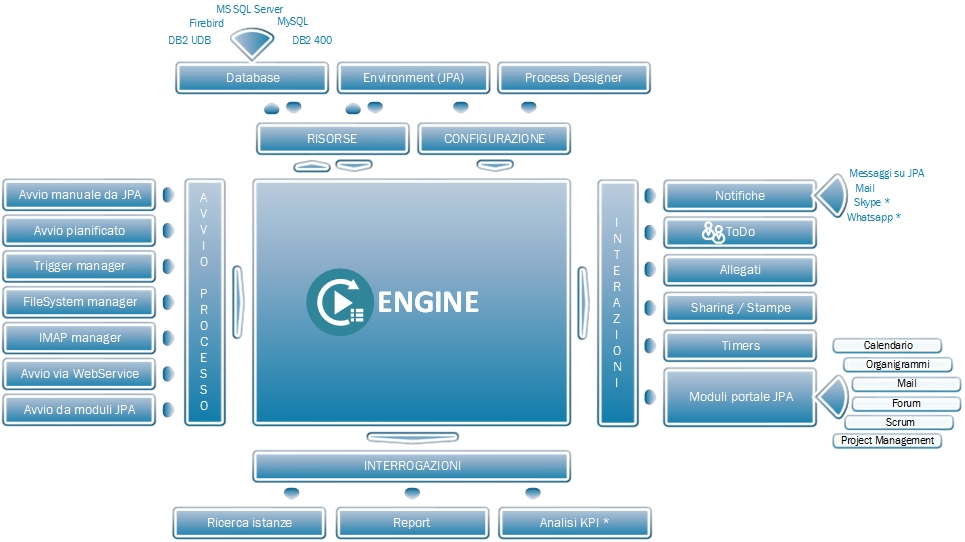
\includegraphics[width=1.25\columnwidth]{immagini/jpa-strutt}%
\caption{Struttura di JPA}%
\label{fig:strutt-jpa}%
\end{figure}
%--------------------------------------------------------------
\subsection{Jgalileo}
Jgalileo è una \gloss{suite} di pacchetti software che messi insieme compongono
un applicativo di tipo gestionale che è in grado di supportare i vari processi
di un'azienda.

Questo \gloss{erp}, prodotto di punta di Sanmarco Informatica, è usato
quotidianamente da più di 1500 aziende, per un totale di oltre 50000 utenti.
Queste aziende operano in diversi mercati: alimentare, commerciale, serramenti,
cantine e distillerie sono solo alcuni di questi.

A seconda delle estensioni (chiamate \textbf{moduli}) richieste dal cliente,
il prodotto può essere specializzato per diverse aree. Alcune di queste sono
amministrazione e finanza, CRM, controllo di gestione, archiviazione
documentale, commerciale, produzione, rilevazione dati, gestione processi,
qualità e business intelligence.

%**************************************************************
\section{Scrum aziendale}

Sanmarco Informatica ha mantenuto fedeltà alla propria \gloss{mission} anche
per quanto riguarda l'organizzazione dei propri processi aziendali.

Al fine di restare attenta alle possibili variazioni delle esigenze dei
clienti, dal 2013 l'azienda ha deciso di abbracciare i principi espressi
nell'\gloss{agilemanifesto}, organizzando i propri team con la metodologia
Scrum.

\subsection{Metodologia Scrum}

Questo approccio è ritenuto un \gloss{framework} dai suoi stessi creatori,
poichè permette di avere notevoli benefici al costo di seguire le sue regole e
le sue linee guida.

La metodologia Scrum infatti rivoluziona l'approccio classico di sviluppo
software a partire dalle sue unità più piccole: i team di sviluppo (in Scrum,
\emph{Development Team}).

Nei progetti ad impostazione ``classica'', un team di sviluppo può avere
composizione variabile a seconda delle persone che ne vengono inserite e
rimosse: tra queste, i ruoli più comuni su cui si basa l'alternanza dei membri
di un gruppo sono analisti, progettisti e programmatori.

In Scrum, la composizione di un team è fissa, poichè un team non cambia
\textbf{mai} i propri componenti se non per cause indipendenti dallo sviluppo
del prodotto su cui il team sta lavorando. Ciò è possibile perchè i
\emph{Development Team} in Scrum sono:

\begin{itemize}
	\item \emph{self-organizing}, ovvero si ripartiscono da soli il lavoro senza
	che un Responsabile di Progetto (o un membro avente funzioni equivalenti a
	questo) assegni loro le attività;
	\item \emph{cross-functional}, in quanto un \emph{Development Team} è nel suo
	complesso competente in tutto ciò di cui necessita per portare a termine un
	progetto.
\end{itemize}

Per quanto si vede nei due punti sovrastanti, è facile notare che i ruoli
classici di progetto scompaiono, o quantomeno vengono gestiti internamente e
flessibilmente all'interno di un team di sviluppo Scrum (termine inglese
utilizzato nel rugby che significa \textbf{mischia ordinata}).

\begin{figure}[H]%
  \noindent\makebox[\columnwidth][c]{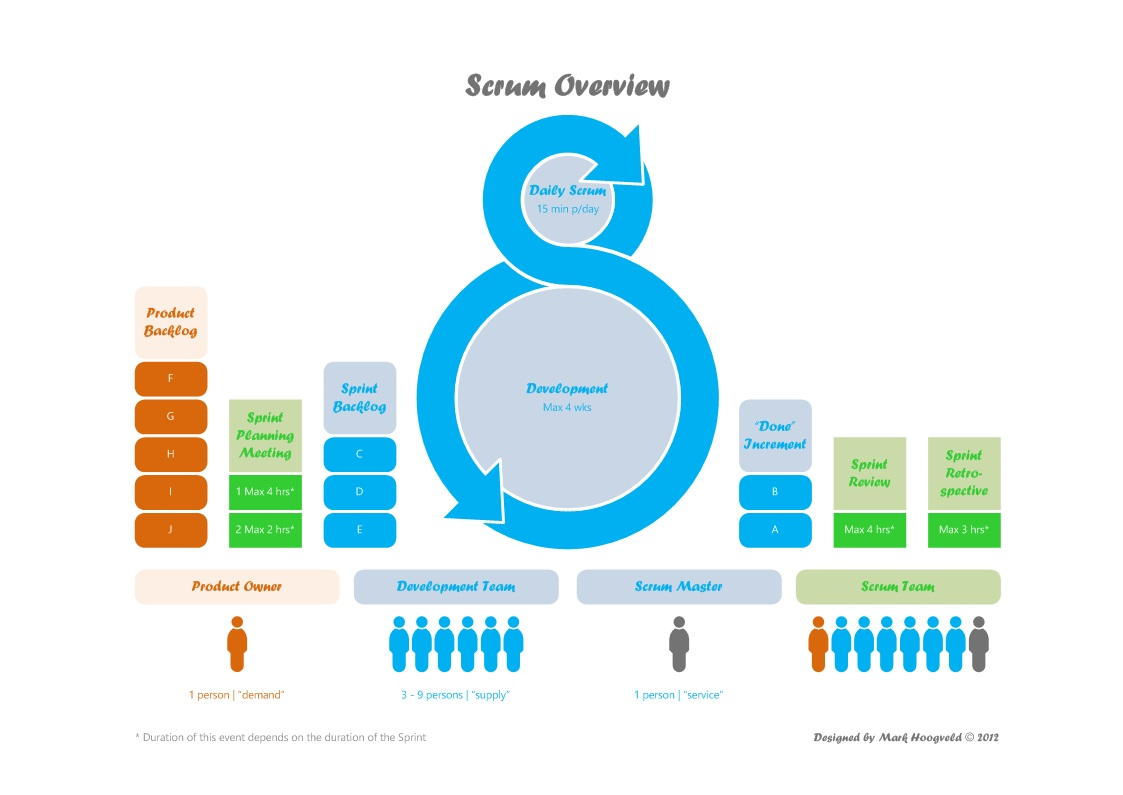
\includegraphics[width=1.5\columnwidth]{immagini/scrum-schema}}%
  \caption{Flusso di sviluppo software in Scrum}%
  \label{fig:scrum-schema}%
\end{figure}%

Un'altra differenza rispetto all'approccio classico dello sviluppo software si
ha nelle misure del team di sviluppo. In Scrum i gruppi hanno dimensione
massima di nove persone, sebbene la dimensione consigliata dagli ideatori sia
di sette membri. Limitando il numero di persone che devono lavorare insieme, la
difficoltà organizzativa viene notevolmente ridotta e il gruppo può
concentrarsi maggiormente sullo sviluppo del prodotto e aver meno problemi
dovuti alla coordinazione interna.

Questo beneficio è ottenibile grazie anche ai due ulteriori ruoli che Scrum
prevede: lo \emph{Scrum Master} ed il \emph{Product Owner}.

Lo \emph{Scrum Master} è la guida dell'intero \emph{Scrum Team} affinchè la
metodologia sia applicata correttamente. Il suo ruolo ha importanza
fondamentale poichè, come riconoscono gli stessi ideatori, Scrum può portare a
conseguenze molto negative se applicato scorrettamente.

Lo \emph{Scrum Master} valuta la qualità dei processi, li ispeziona e fornisce
al resto del gruppo soluzioni per diminuire gli sprechi di risorse e
massimizzare il valore delle interazioni tra i componenti del gruppo.

Il \emph{Product Owner} consente invece al \emph{Development Team} di
continuare lo sviluppo del prodotto senza continue interruzioni dovute
al dialogo con i portatori di interesse (\emph{stakeholders}) esterni allo
\emph{Scrum Team} o alla continua variazione dei requisiti.

Egli è responsabile del carico di lavoro (chiamato \emph{backlog}) presente per
il \emph{Development Team} e si interfaccia costantemente con quest'ultimo per
determinare la priorità e stimare lo sforzo necessario per portare a termine
ciascun task, ovvero un'attività il cui completamento comporta il
soddisfacimento di un requisito utente.

Scrum mantiene fede a uno degli obiettivi principali dei metodi agili, ovvero
tenere alto il coinvolgimento del cliente: questa metodologia, infatti, dispone
di un modo efficiente per verificare frequentemente che ciò che viene prodotto
dal \emph{Development Team} risponda correttamente alle necessità del cliente.

I task vengono infatti inseriti in cicli produttivi chiamati \textbf{sprint},
aventi durata massima un mese (dalla loro brevità deriva il termine
``sprint''), al termine dei quali viene presentato al cliente un incremento
potenzialmente rilasciabile.

All'inizio di ogni sprint vi è una \gloss{cerimonia} chiamata \emph{Sprint
Planning}, con la quale vengono decisi quali task il \emph{Development Team}
ritiene di riuscire a portare a termine nel prossimo sprint, dialogando con il
\emph{Product Owner} affinchè venga data precedenza ai task con maggiore
priorità per il cliente.

L'arco temporale ristretto in cui uno sprint è contenuto permette al
\emph{Development Team} di rispondere velocemente a variazioni dei requisiti:
sebbene durante lo sprint il team di sviluppo si concentri esclusivamente sui
task concordati nell'attività di \emph{Planning}, il tempo che scorre
dall'inizio sprint alla sua fine è sufficientemente ridotto per evitare che
eventuali task urgenti inseriti nel frattempo nel \emph{backlog} rimangano
ignorati per tempi eccessivi.

In ciascun giorno dello sprint, viene tenuta una \gloss{cerimonia} chiamata
\emph{Daily Scrum}. In questa occasione, i membri del \emph{Development Team}
espongono cosa hanno fatto nel giorno precedente, cosa faranno nel giorno
corrente e quali problemi hanno incontrato durante lo svolgimento dei task.

Una volta terminato lo sprint, vi sono due \glosspl{cerimonia}.

La prima, a cui partecipa anche il cliente, è chiamata \emph{Sprint Review} e
serve a presentare un incremento potenzialmente rilasciabile. Grazie
a questi incontri viene incentivata l'interazione tra fornitore e cliente,
fattore spesso alla base della buona riuscita di progetti di sviluppo software.

La seconda \gloss{cerimonia} di fine sprint si chiama \emph{Sprint
Retrospective} e consente al gruppo di analizzare le opinioni ricevute dal
cliente e di lavorare nell'ottica del miglioramento continuo. Vengono infatti
discussi a fondo quali sono i cambiamenti che il team potrebbe attuare ai
propri processi, per ridurne i costi o per riuscire a fornire al cliente un
prodotto che risponda maggiormente alle sue esigenze.
%**************************************************************
\section{Tecnologie utilizzate}

Sanmarco Informatica usa diverse tecnologie, sia a supporto dei processi
aziendali che per lo sviluppo di JPA.

\subsection{JPA}

L'area Scrum di JPA è utilizzata costantemente dal team in cui sono stato
inserito.

Quest'area dell'applicazione offre infatti supporto all'organizzazione di
sprint e all'assegnazione dei task in esso contenuti.

Gli sprint sono infatti visualizzati in un'interfaccia facilmente comprensibile
anche a chi è estraneo a Scrum, che rende agevole la gestione dei task presenti
nello sprint backlog.

\begin{figure}%
  \noindent\makebox[\columnwidth][c]{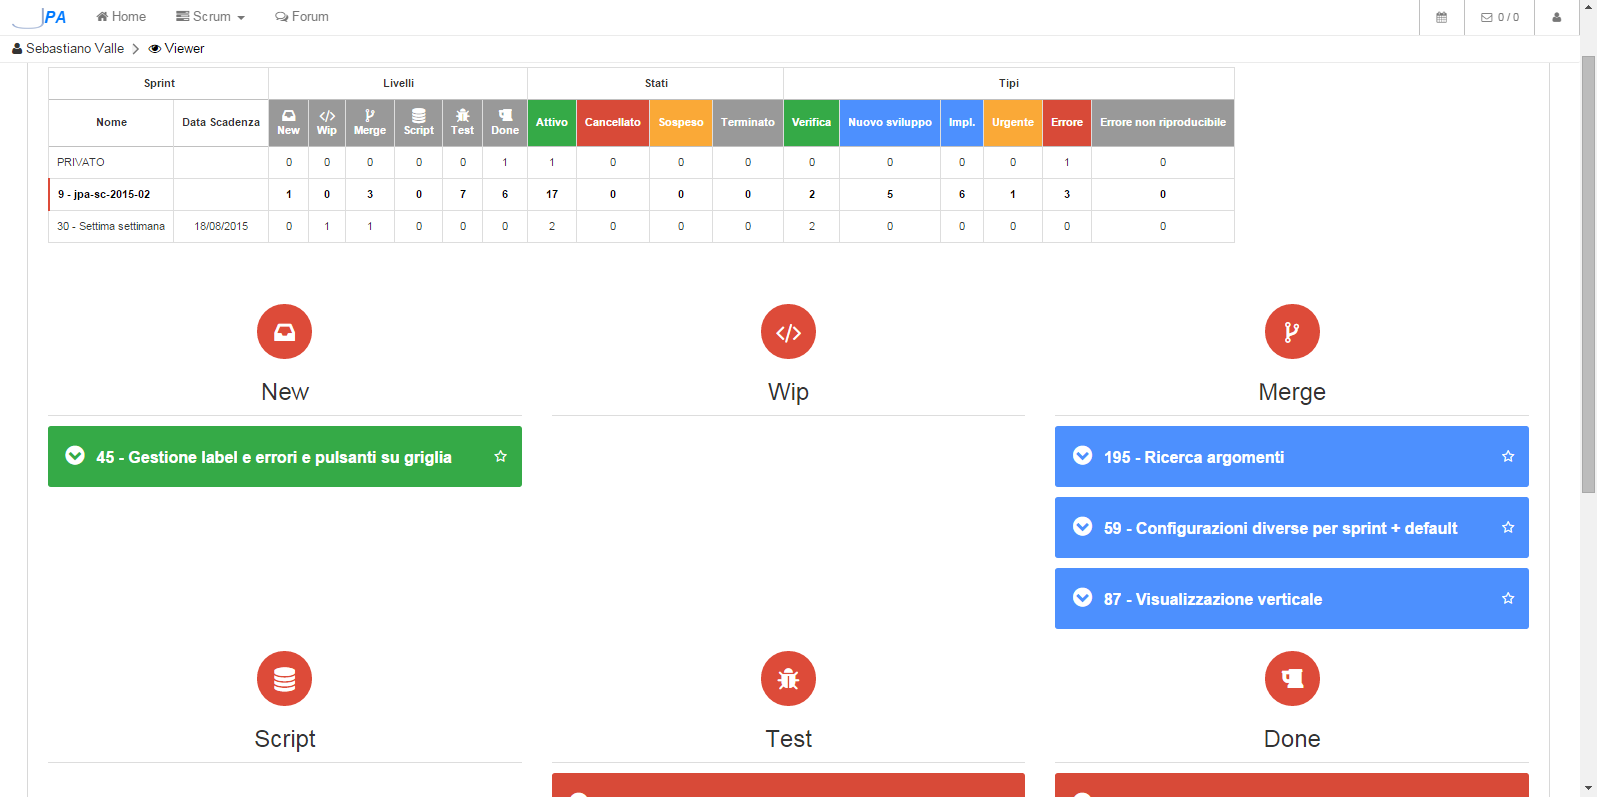
\includegraphics[width=1.3\columnwidth]{immagini/jpa-sprint-viewer}}%
  \caption{Schermata di visualizzazione sprint in JPA}%
  \label{fig:jpa-viewer}%
\end{figure}

Come è possibile vedere in figura \ref{fig:jpa-viewer}, i task possono essere
in diversi livelli a seconda del loro stato di avanzamento.

Questi livelli sono configurabili dall'amministratore di sistema e nel mio team
un task può passare per i seguenti stadi:

\begin{itemize}
	\item \textbf{New}, quando nessuno ha lavorato sul task e questo è ancora in
	analisi;
	\item \textbf{Wip}, quando uno o più membri del gruppo stanno lavorando sul
	task;
	\item \textbf{Merge}, in cui l'incremento dovuto al task viene integrato a
	JPA;
	\item \textbf{Script}, quando una modifica deve essere integrata tramite
	script (ad esempio l'inserimento di una riga in database);
	\item \textbf{Test}, in cui l'incremento prodotto dallo svolgimento del task
	viene controllato da un altro membro del gruppo;
	\item \textbf{Done}, in cui l'incremento prodotto da un task è definitivamente
	approvato ed integrato in JPA.
\end{itemize}

\begin{figure}[H]%
  \noindent\makebox[\columnwidth][c]{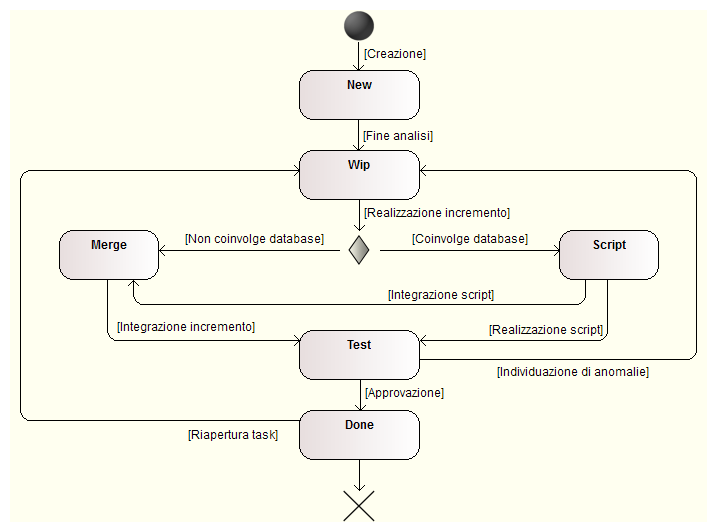
\includegraphics[width=1.1\columnwidth]{immagini/task-life-cycle}}%
  \caption{Ciclo di vita di un task}%
  \label{fig:task-lifecycle}%
\end{figure}

Oltre a questi livelli, è necessario indicare il \textbf{tipo} di un task, a
seconda della sua natura (Nuovo sviluppo, Implementazione, Urgente, Errore,
Errore non riproducibile).

Ogni task può essere preso in carico da uno o più operatori e vi si possono
aggiungere note o file in allegato.

\paragraph{Sprint privati} \mbox{}

JPA offre anche la possibilità di creare sprint privati, visibili solamente
all'utente che li ha creati, in cui vanno inseriti le attività di minore
importanza o dei task usati come promemoria.

\paragraph{Fine sprint} \mbox{}

Al termine di uno sprint, vi sono tre alternative possibili per ciascun task:

\begin{itemize}
	\item se un task è nello stato Done, è ritenuto concluso e JPA lo ignora;
	\item se un task è nello stato New, questo può essere assegnato ad un altro
	sprint o rimanere senza sprint;
	\item se un task è in uno dei rimanenti stati, \textbf{deve} essere
	riassegnato ad un altro sprint.
\end{itemize}

\subsection{JPADb}

JPADb è il database su cui JPA si appoggia. Tale base dati può essere gestita
da uno dei seguenti \gloss{rdbms}: MySQL, Firebird, DB2 400, MS SQL Server e DB2
UDB.

Le alterazioni alle tabelle o al loro contenuto avvengono tramite script Java,
utilizzando funzionalità del package \texttt{java.sql}.

Sebbene possa sembrare difficile applicare una modifica vista la diversa natura
dei vari \gloss{rdbms}, questo lavoro è notevolmente semplificato grazie ad
alcune \gloss{api} di JPA che consentono di eseguire i comandi di alterazione
delle tabelle e del loro contenuto in puro linguaggio SQL.

In questo modo lo sviluppatore può non essere a conoscenza dei dettagli di ogni
specifico sistema ed evitare di dover realizzare soluzioni complesse per delle
semplici operazioni come la creazione di una tabella ogni volta che si presenta
la necessità di compiere questo tipo di azione.

\paragraph{Norme e raccomandazioni per lo sviluppo} \mbox{} \\

Al momento del mio ingresso nel team, sono presenti le seguenti norme per la
creazione di tabelle in JPADb:

\begin{itemize}
	\item i nomi delle tabelle devono sempre riferirsi al plurale, in lingua
	inglese, agli elementi in essa contenuti. Eventuali deviazioni da tale regola
	devono essere discusse;
	\item i nomi delle tabelle devono sempre contenere il codice dell'area in cui
	vengono utilizzate come prefisso prima del nome degli elementi che questa
	contiene;
	\item una \gloss{chiaveprimaria} deve iniziare con \texttt{SEQ\_} e finire
	con il nome della tabella a cui è associata;
	\item una chiave esterna deve iniziare con \texttt{FK\_}, proseguire con il
	codice dell'area in cui viene utilizzata e un numero progressivo per
	distinguerla dalle altre della stessa area.
\end{itemize}

\subsection{Back-end}

Il lato server di JPA è realizzato con il linguaggio di programmazione Java.
Il \BKEND{} si decompone in \emph{WebServices} e \emph{WebShared}, per riuscire
rispettivamente ad accogliere le richieste dal client e delegarle al servizio
più adeguato.

Nella parte di \emph{WebServices} si trovano delle classi utilizzate per
accogliere le chiamate \gloss{rest} che provengono dal lato client. Per gestire
tali servizi, vengono utilizzate le \gloss{jaxrs} Jersey.

Affinchè i \emph{WebServices} siano leggeri e facilmente ritoccabili, tutta la
\emph{business logic} viene spostata nella parte di \emph{WebShared}, che
interagisce direttamente col database.

La parte di \emph{WebShared} non comunica direttamente con il client: per
questo motivo, i risultati delle operazioni sul database vengono consegnati
alla parte di \emph{WebServices} che si occupa di trasmetterli al \FREND{}.

JPA viene avviato e caricato sull'\gloss{applicationserver} Tomcat, il quale
viene a sua volta eseguito su una macchina virtuale le cui copie sono
utilizzate da tutti i membri del team.
La codifica, l'avvio dei server e il versionamento del codice avvengono
all'interno dell'\gloss{ide} Eclipse.

\paragraph{Versionamento} \mbox{} \\

La parte di \BKEND{} di JPA è versionata con il \gloss{vcs} SVN. Non vengono usati
particolari flussi di sviluppo, dal momento che tutte le modifiche vengono
applicate direttamente al ramo principale (\emph{trunk}) del
\gloss{repository}.

Ad ogni integrazione di una modifica al ramo principale, è obbligatorio
inserire un breve commento che descriva il cambiamento effettuato.

\paragraph{Norme e raccomandazioni per lo sviluppo} \mbox{} \\

Per quanto riguarda il lato server di JPA, gli sviluppatori sono tenuti a
seguire queste norme:

\begin{itemize}
	\item se una classe dei \emph{WebServices} fa parte di un'area (e.g.
	Scrum, avente codice \texttt{Sc}), il suo nome dovrà cominciare con il
	codice di questa;
	\item i metodi delle classi dei \emph{WebServices} devono essere statici;
	\item I metodi delle classi dei \emph{WebServices} devono avere dimensione
	ridotta (al massimo 20 righe), così da essere facilmente modificabili;
	\item gli URL che identificano i metodi della parte di \emph{WebServices}
	devono essere costituiti da insiemi di lettere lunghi al massimo tre
	lettere\footnote{Ad esempio il metodo \texttt{getList()} di una classe
	\texttt{ScSprint} nel package \texttt{plugins.sc} avrà un URL come
	\texttt{ws/pl/sc/s/l}, o simile}. Tale norma è legata a motivi di efficienza
	nell'eseguire chiamate \gloss{rest} al \BKEND{};
	\item usare sempre l'annotazione \texttt{@Override} quando una classe
	ridefinisce o concretizza un metodo della classe che estende o
	dell'interfaccia che implementa;
	\item usare sempre i metodi forniti dalle \gloss{api} di JPA per connettersi al
	database e chiudere la connessione a questo;
	\item il tempo di esecuzione di un metodo dei \emph{WebServices} deve essere
	sempre misurato;
	\item far corrispondere ad ogni classe \texttt{MyClass} nei
	\emph{WebServices} una classe \texttt{MyClassUtil} nella parte di
	\emph{WebShared} che soddisfi le richieste \gloss{rest} ricevute da
	\texttt{MyClass};
	\item ogni classe nella parte di model nei \emph{WebShared} deve avere il
	prefisso \texttt{Def};
	\item ogni metodo di una classe deve essere scritto rispettando le seguenti
	regole di stile:
	\begin{enumerate}
		\item le righe di istruzioni di importazione di package devono essere
		ordinate in ordine alfabetico;
		\item tra il nome di un metodo e le sue parentesi deve esserci uno spazio;
		\item le righe di codice vanno indentate;
		\item non bisogna usare il carattere di tabulazione per l'indentazione ma
		quattro spazi;
		\item è obbligatorio lasciare una riga vuota tra un metodo e l'altro;
		\item i nomi di classi devono essere scritti in \emph{UpperCamelCase};
		\item i nomi di metodi ed attributi devono essere scritti in
		\emph{lowerCamelCase};
		\item i nomi dei campi di un tipo enumerativo devono essere scritti in
		\emph{SNAKE\_CASE}, con tutti i caratteri in maiuscolo;
		\item ogni classe e ogni metodo devono avere il proprio nome aggiunto come
		commento nella linea in cui terminano.
	\end{enumerate}
\end{itemize}

Oltre alle regole sopra elencate, vi sono le seguenti raccomandazioni:

\begin{itemize}
	\item usare metodi statici anche nelle classi dei \emph{WebShared}, qualora
	possibile;
	\item commentare le parti di codice più complesse.
\end{itemize}

\paragraph{JPAUtil} \mbox{} \\

Nella parte di JPA dedicata alla modellazione di processi sono presenti
alcune \gloss{api} di utilità generica. Tali funzioni sono visibili a chi modella
un processo, la cui preparazione informatica può anche essere basilare.

Queste funzioni possono essere collegate ad un evento, ad esempio
l'approvazione di una richiesta di acquisto nella modellazione di un processo.

Per questo motivo, il team ha adottato le seguenti norme:

\begin{itemize}
	\item ogni funzione fornita da una \gloss{api} in JPAUtil deve verificare se
	la connessione al database è già aperta\footnote{Tale controllo alleggerisce
	notevolmente le responsabilità all'utilizzatore delle \gloss{api}}:
	\begin{itemize}
		\item Nel caso in cui lo fosse, utilizzare la connessione al database già
		esistente senza chiuderla al termine dell'operazione;
		\item Nel caso in cui non lo fosse, aprirne una propria e chiuderla al
		termine dell'operazione.
	\end{itemize}
	\item ad ogni metodo pubblico al quale viene richiesta un'operazione, ne deve
	corrispondere uno che esegue l'operazione richiesta;
	\item i metodi pubblici devono avere come \textbf{ultimo} parametro formale
	un oggetto di tipo \texttt{Connection}, mentre i metodi privati devono avere
	tale oggetto come \textbf{primo} parametro.
\end{itemize}

Siccome l'utilizzatore di queste \gloss{api} potrebbe disporre di una
preparazione informatica basilare, è raccomandato di preferire l'aggiunta di
parametri all'incapsulamento di questi in una classe.

Ciò è dovuto al fatto che molti possibili clienti dell'azienda potrebbero
non conoscere la programmazione ad oggetti e potrebbe risultare più facile per
questi elencare gli attributi di un oggetto piuttosto che far propri i
fondamenti di informatica necessari.

\subsection{Front-end}

Il lato client di JPA consiste in una \gloss{spa} realizzata con diverse
tecnologie:

\begin{itemize}
	\item HTML5 per la componente strutturale e semantica della pagina. Tale
	linguaggio è raccomandato dal \gloss{w3c} da ottobre 2014.
	\item TODC Bootstrap, un \gloss{framework} open source derivato da Bootstrap
	di Twitter. Sviluppato da una comunità di designer web, usa CSS3 e fornisce
	uno stile alle pagine simile a quello di Google;
	\item AngularJS, un \gloss{framework} che guida lo sviluppo di \gloss{spa}
	con elementi architetturali che si ispirano al pattern MVC.
\end{itemize}

Il browser su cui viene provata JPA è Chromium, mentre il codice del \FREND{}
viene scritto utilizzando Sublime Text 2.

L'applicazione \FREND{} di JPA al momento ha come lingue disponibili l'italiano
e l'inglese. Tuttavia l'aggiunta di nuovi dizionari è semplice poichè i testi
delle viste HTML sono gestiti in modo automatico da JPA tramite un dizionario.

\paragraph{Versionamento} \mbox{} \\

A differenza del \BKEND{}, il lato client non dispone di un \gloss{vcs}.

Per questo motivo, quando gli incrementi per il \FREND{} vengono sviluppati,
vanno allegati in JPA passando al livello Merge in modo tale che possano essere
integrati in JPA da Alex Beggiato, una volta testati.

Non essendovi un \gloss{repository} di accesso comune, i file utilizzati vengono
distribuiti ad intervalli non definiti, solitamente quando un membro deve
effettuare una modifica su una parte su cui un altro componente del team ha
cambiato parte del codice.

Nel caso in cui due persone avessero modificato lo stesso file nel \FREND{}, si
raccomanda di usare \textbf{Meld} per unire i due file, anche se ciascun
componente del team è libero di utilizzare lo strumento che preferisce.

\paragraph{Norme e raccomandazioni per lo sviluppo} \mbox{} \\

Al momento del mio ingresso nel team, sono presenti le seguenti norme per lo
sviluppo del lato client di JPA:

\begin{itemize}
\item ogni variabile locale ad una funzione deve essere preceduta dalla parola
chiave \texttt{var} nella sua dichiarazione, poichè vengono utilizzate diverse
variabili e funzioni globali;
\item le parti di testo visualizzate in JPA sono proprietà dell'oggetto
\texttt{\$scope.\_label} e devono essere lette con la funzione
\texttt{\_getLabelFor()}, la quale a sua volta utilizza dei file di
configurazione contenenti delle parole o delle frasi in diverse lingue;
\item ogni statement deve essere concluso con un punto e virgola;
\item assegnare un codice univoco ad ogni errore. L'ultimo codice di errore
utilizzato per una certa area è riportato nell'area Forum di JPA;
\item in ogni chiamata che esegue una chiamata \gloss{rest} verso il \BKEND{},
impedire l'uso della pagina all'utente  mostrando una schermata di attesa fino
al termine dell'operazione;
\item anteporre \texttt{data-} ai nomi delle direttive di AngularJS nei tag
HTML;
\item i nomi delle funzioni devono cominciare con ``\texttt{on}'' se invocate
direttamente da un elemento della vista HTML.
\end{itemize}

\section{Propensione all'innovazione}

Sanmarco Informatica compie molti sforzi per rimanere aggiornata ed essere
innovativa e competitiva sul mercato.

\subsection{Investimento nella ricerca} \mbox{}

Durante il periodo del mio stage ho lavorato al centro aziendale di Ricerca,
Sviluppo e Formazione. In questa sede, oltre al miglioramento e alla
manutenzione di funzionalità già presenti nei software in commercio, vengono
svolte anche attività di ricerca e prototipazione (come è successo nel caso
del mio stage).

L'azienda procede in modo deciso in questa direzione: l'investimento medio del
proprio fatturato in ricerca da quando l'azienda è nata corrisponde al 17\%,
mentre negli ultimi due anni (2013 e 2014) è arrivato al 20\% per ciascun anno.

Questa scelta ha portato i suoi benefici, aiutando l'azienda ad avere dei
risultati economici nettamente in contrasto con l'andamento del resto
dell'economia nazionale: il bilancio del 2014 si è chiuso con un incremento del
34\%, mentre la crescita prospettata per la fine del corrente anno è del 40\%.

I guadagni ottenuti hanno consentito all'azienda di investire anche assumendo
13 nuovi dipendenti, di cui 5 ricercatori.

\subsection{OpenPOWER Foundation} \mbox{}

Sanmarco Informatica è la prima ed unica azienda italiana che è entrata a far
parte (ad inizio 2015) della prestigiosa fondazione \textbf{OpenPOWER
Foundation}.

Tale consorzio, creato da Google, IBM, Mellanox Technologies, Tyan, Samsung e
Nvidia è una comunità i cui partner collaborano per ricavare un'opportunità di
crescita e riuscire ad adeguarsi all'evoluzione dei bisogni dei clienti.
Questo obiettivo viene raggiunto da OpenPOWER Foundation condividendo
competenze e investimento nella ricerca da parte di aziende ed università.

Entrando in OpenPOWER Foundation, Sanmarco Informatica ha deciso di offrire il
suo contributo sviluppando PowerJ (una nuova versione di Jgalileo), un
\gloss{erp} basato su tecnologie open source, in grado di offrire risparmi in
costi di licenza, preferendo tecnologie opensource ad alternative proprietarie.

Con questo prodotto il cliente può disporre del cosiddetto sistema ``Cloud On
Site'': PowerJ semplifica l'uso di una piattaforma Cloud proteggendo i dati ed
integrando le applicazioni sulla piattaforma Cloud con quelle in locale.


\begin{figure}[H]%
  \noindent\makebox[\columnwidth][c]{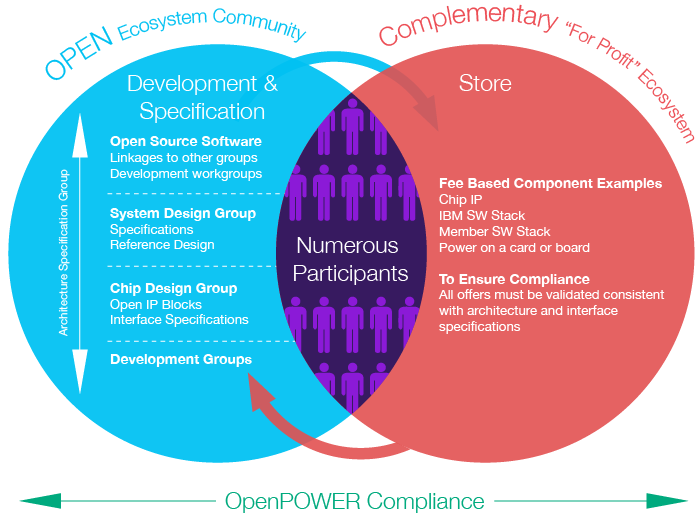
\includegraphics[width=\columnwidth]{immagini/open-power-foundation}}%
  \caption{Ciclo di vita di un task}%
  \label{fig:task-lifecycle}%
\end{figure}

\subsection{4words} \mbox{}

La propensione all'innovazione di Sanmarco Informatica è confermata anche
dall'esistenza di progetti come \textbf{4words}, web agency che prende il suo
nome da quattro valori a cui dichiara di ispirarsi: efficacia, funzionalità,
flessibilità e innovazione.

Questo team si occupa principalmente di realizzazione di siti Web e promozione
online per aziende. Grazie ai suoi servizi, le aziende riescono a guadagnare
visibilità rispetto al consumatore, migliorando l'efficacia del proprio sito in
termini di indicizzazione da parte di Google (\textbf{SEO}) e promuovendo il
proprio marchio nei social network.

Al momento il progetto si sta muovendo verso il futuro cercando di anticipare
l'evoluzione dei motori di ricerca. Per far ciò, uno degli obiettivi attuali
del progetto è costruire delle mappe linguistiche che possano essere integrate
nei siti favorendo l'indicizzazione semantica e permettendo di farsi trovare
più facilmente dall'utente.

\subsection{Prodotti} \mbox{}

Sanmarco Informatica si propone in modo innovativo al cliente anche per quanto
riguarda alcune delle tecnologie che utilizza per sviluppare i propri prodotti.

La decisione dell'azienda è ambiziosa e al contempo coraggiosa: i prodotti che
offre gestiscono la pianificazione delle risorse di aziende, un campo dove
errori o comportamenti inattesi dovuti a tecnologie poco stabili possono
costare molto.

Sanmarco Informatica agisce sviluppando soluzioni che siano robuste e stabili
sul lato server dei propri software, affidandosi a un colosso dell'informatica
come IBM e a tecnologie stabili ed affermate come Java e SQL.

Allo stesso tempo, si mantiene moderna sperimentando vari modi per far
interagire gli utenti con le proprie applicazioni: le tecnologie utilizzate (ad
esempio AngularJS) spesso sono molto giovani e sono soggette al rischio di
mutazioni drastiche nel giro di brevi periodi.

L'azienda non trascura il mondo \emph{mobile}: le applicazioni Web sono
\gloss{responsive} e vi sono progetti che si occupano esclusivamente dello
sviluppo di applicazioni per smartphone e tablet.

\subsection{Personale} \mbox{}

Quanto visto per le tecnologie utilizzate per i propri prodotti si riflette sul
personale all'interno dell'azienda, che combina saggiamente esperienza con le
menti fresche di giovani, provenienti sia da scuole superiori che da
università.

Ogni anno Sanmarco Informatica offre infatti molteplici opportunità di attività
di stage, nelle quali i giovani possono dare il loro contributo alla software
house potendo lavorare su tecnologie accattivanti ed al contempo guadagnado
utile esperienza.

\subsection{Scrum} \mbox{}

Un ulteriore aspetto in cui si può notare la propensione all'innovazione di
Sanmarco Informatica sta nel fatto di aver adottato la metodologia Scrum.

Non era scontato che un'azienda operante da circa venticinque anni che produce
software gestionale decidesse di cambiare il modello con cui i processi e le
persone sono organizzate per lo sviluppo dei propri prodotti.

Questa scelta coraggiosa ha rinfrescato l'azienda, snellendo i processi e ha
permesso di riuscire meglio nel rispettare scadenze e a far fronte a
tempistiche pressanti.
             % Introduzione
% !TEX encoding = UTF-8
% !TEX TS-program = pdflatex
% !TEX root = ../tesi.tex
% !TEX spellcheck = it-IT

%**************************************************************
\chapter{Strategia aziendale}
\label{cap:strat-aziend}
%**************************************************************

\intro{Questo capitolo serve per descrivere come l'azienda percepisce le
attività di stage e come le gestisce, parlando in particolare dello stage a
cui la relazione finale fa riferimento.}\\

%**************************************************************
\section{Il progetto}\label{sec:strat-prog}

Il progetto di stage era rivolto all'estensione dell'area Scrum di JPA.

Tale area, nata grazie ad un'altra attività di stage, viene utilizzata
quotidianamente dal team in cui sono stato inserito.

Il mio compito durante l'attività di stage è stato aggiungere funzionalità
che rendessero più soddisfacente l'uso dell'area Scrum di JPA. Questo è stato
possibile riconoscendo alcuni limiti che ad inizio stage JPA presentava:

\begin{itemize}
\item Per poter essere utilizzato da team che adottano la metodologia Scrum,
  vi era la necessità di studiare le differenze tra quanto previsto da Scrum e
  quanto offerto attualmente da questa area di JPA;
\item La decomposizione dei task più complessi era frequentemente fonte di
  problemi, siccome rendeva poco comprensibile il visualizzatore di sprint per
  le seguenti cause:
  \begin{itemize}
  \item Il meccanismo già presente per dire che un task è padre di un altro non
    consentiva una visione chiara della relazione, che non veniva evidenziata
    nel visualizzatore di sprint;
  \item Sia esplicitando la relazione padre-figlio tra diversi task che
    evitando di farlo, per suddividere un task in più sotto-task dovevano
    essere create \textbf{molte} attività, che compromettevano la leggibilità
    del visualizzatore di sprint.
  \end{itemize}
\item Nonostante uno dei principi fondamentali di Scrum sia l'\emph{Inspection}
  dei propri processi, non vi era nessuno strumento a sostegno della verifica
  e il controllo dei propri processi;
\item Ai clienti che fanno uso delle aree di modellazione processi di JPA
  potrebbe servire un collegamento tra queste e l'area Scrum;
\item L'area Scrum di JPA prevedeva esclusivamente il \emph{pull model} come
  modalità per ottenere informazioni: questo problema incideva chiaramente
  sull'efficienza del team, dal momento che non era possibile ottenere
  informazioni se non per controllo manuale da parte degli utenti.
\end{itemize}

In tabella \ref{tab:piano-di-lavoro} è riportato il Piano di Lavoro previsto
inizialmente per le otto settimane di stage: \\

\begin{tabular}{| c | p{10cm} |}

\hline
\textbf{Settimana} & \textbf{Lavoro previsto} \\
\hline
1 & Ricerca, studio e documentazione sulla metodologia scrum. Introduzione
    ai linguaggi di sviluppo. Analisi dello stato attuale del prodotto e
    confronto con la parte teorica. \\
\hline
2 & Analisi iniziale sulla gestione delle checklist legate ai task.
    Sviluppo modulo anagrafico di gestione checklist. Documentazione modulo
    anagrafico di gestione checklist. \\
\hline
3 & Sviluppo gestione checklist legate ai task. Documentazione relativa. \\
\hline
4 & Analisi su come produrre il burn-down chart con i dati presenti a
    sistema. Analisi ed eventuale sviluppi sui dati mancanti e necessari
    alla produzione del burn-down chart. Inizio sviluppo modulo di
    configurazione chart. \\
\hline
5 & Eventuale completamento del modulo di configurazione chart. Sviluppo e
    documentazione del burn-down chart. \\
\hline
6 & Completamento documentazione e tesi con obiettivi raggiunti e spunti
    per possibili altri sviluppi futuri. Analisi, sviluppo e
    documentazione gestione avvio istanza da task scrum. \\
\hline
7 & Analisi, sviluppo e documentazione sul collegamento tra modulo scrum e
    modulo di notifica. \\
\hline
8 & Analisi, sviluppo e documentazione sul collegamento tra modulo scrum e
    modulo forum. \\
\hline
\end{tabular}
\captionof{table}{Piano di Lavoro}
\label{tab:piano-di-lavoro}

%**************************************************************
\subsection{Il progetto visto dall'azienda}\label{sec:strat-ob-prod}

Questo stage avrebbe portato all'azienda diversi vantaggi, distinti in
obiettivi (produttivi) minimi e massimi. Sia che fossero minimi che massimi,
entrambi i tipi di obiettivi prevedevano la stesura di documentazione per
quanto sarebbe stato prodotto durante l'attività di stage. \\

\begin{tabular}{| p{6cm} | p{6cm} |}

\hline
\textbf{Obiettivi minimi} & \textbf{Obiettivi massimi} \\
\hline
Confronto tra stato attuale di JPA e Scrum ``puro'' &
Avvio di un'istanza di processo da un task \\
\hline
Sviluppo di un modulo di checklist &
Sviluppo di un sistema di notifiche push \\
\hline
Sviluppo di una \gloss{direttiva} per visualizzare un burn-down chart per uno
  sprint &
Collegamento tra area Scrum e Forum \\
\hline
\end{tabular}
\captionof{table}{Obiettivi produttivi}
\label{tab:obiettivi-produttivi}

%**************************************************************
\subsection{Il progetto visto dallo stagista}

L'attività di stage è inserita nel piano di studi di un Corso di Laurea.

Proprio per questo motivo, il Piano di Lavoro è stato pensato affinchè io
riuscissi a guadagnare qualcosa dallo stage: sono stati infatti individuati
degli obiettivi (formativi) minimi e massimi. \\

\begin{tabular}{| p{6cm} | p{6cm} |}

\hline
\textbf{Obiettivi minimi} & \textbf{Obiettivi massimi} \\
\hline
Ottenimento di una conoscenza profonda di Scrum &
Capacità di adattare i principi di Scrum ad esigenze diverse dallo sviluppo
  software \\
\hline
Acquisizione delle competenze necessarie per sviluppare le funzionalità
  previste negli obiettivi produttivi &
\mbox{} \\
\hline
\end{tabular}
\captionof{table}{Obiettivi formativi}
\label{tab:obiettivi-formativi}

\paragraph{La scelta} \mbox{} \\

Prima dello stage la mia conoscenza sull'azienda era limitata e di Jgalileo
sapevo solamente pochi dettagli.
L'incontro avvenuto a
Stage-IT\footnote{\url{http://informatica.math.unipd.it/laurea/stageit.html}}
mi ha permesso di conoscere meglio la realtà aziendale e di richiedere un
progetto che potesse includere lo studio di Scrum, siccome i metodi agili
costituiscono un campo di studio molto coinvolgente per me.

Qualche decennio fa i metodi con impostazione classica trovavano spazio
e efficacia di applicazione, siccome il software era potenzialmente
assimilabile ad un'attività di tipo industriale, dove requisiti e architettura
vengono stabiliti inizialmente e mantenuti per mesi, fino ad una nuova analisi
di mercato.

Con l'avvento della globalizzazione non sempre è possibile applicare questi
metodi, vista la mutevolezza del mondo esterno e dei suoi bisogni. Per questo
motivo, ritengo che lo studio e l'applicazione di Scrum e altri metodi
agili possa essere determinante per evitare il fallimento di progetti
software.

Oltre alla tematica principale dello stage, altri motivi che mi hanno portato
a questa scelta sono:

\begin{itemize}
\item Conoscere parte del mondo dei software gestionali;
\item Lavorare in un ambiente giovane, con molte persone al suo interno;
\item Poter contribuire direttamente all'efficienza dei processi aziendali;
\item Poter lavorare su una web application con tecnologie a me nuove.
\end{itemize}

%**************************************************************
\section{Come l'azienda usa gli stage}

Sanmarco Informatica, come detto nel primo capitolo, fornisce diverse
opportunità di stage, a seconda della provenienza dei tirocinanti (scuole
superiori, università o altro).

È di particolare interesse comprendere come queste attività vengano adoperate
dall'azienda per formare tali risorse o ottenere benefici dal lavoro di queste
nel breve periodo e, nel secondo caso, il valore aggiunto che questi benefici
portano.

%**************************************************************
\subsection{Visione dell'attività stage}

\paragraph{Formazione} \mbox{} \\

Mentre per gli stage di diversa natura (e.g. scuole superiori o iniziative
indipendenti da istituzioni scolastiche) le risorse sono sottoposte a dei
corsi di formazione che spesso partono dai fondamenti della programmazione ad
oggetti, nel caso degli stage per studenti al termine degli studi di
Informatica non è previsto nessun corso iniziale da parte di personale
aziendale.

Tuttavia, non avendo conoscenze approfondite su tecnologie e metodologie usate
dal team in cui sono stato inserito, la prima settimana è stata dedicata allo
studio e all'approfondimento (come indicato in tabella
\ref{tab:piano-di-lavoro}) come preparazione per le successive settimane.

\paragraph{Benefici derivanti dallo stage} \mbox{} \\

La forza-lavoro di cui un'azienda dispone grazie alle attività di stage può
essere utilizzata in diversi modi.

Per quanto riguarda Sanmarco Informatica, vi sono principalmente tre visioni
sull'attività di stage: una volta alla formazione, una alla prototipazione e
una terza dedicata allo sviluppo.

Come detto precedentemente, gli stage fortemente orientati alla formazione
sono riservati a coloro che non dispongono di un ricco background informatico,
in modo tale da permettere loro di acquisire le competenze necessarie per
poter lavorare in una software house che sviluppa \gloss{erp}.

Il secondo modo in cui l'azienda usa gli stage è per prototipazione: in questo
caso lo stagista prova a percorrere strade potenzialmente utili al resto del
team, sebbene non vi sia la garanzia che il prototipo prodotto venga
effettivamente integrato in un secondo momento.

Questa alternativa è dovuta al fatto che molte volte il team già inserito in
azienda non ha tempo per sperimentare nuove soluzioni, nonostante queste
potrebbero portare notevoli benefici.

Infine, Sanmarco Informatica può utilizzare gli stage per lo sviluppo di nuove
funzionalità in prodotti già esistenti, come nel mio caso.

Durante la mia permanenza in azienda, ho potuto infatti vedere JPA evolversi
grazie al mio contributo.

Un altro vantaggio derivante da questo tipo di stage è il carico di
responsabilità attribuitami: eventuali difetti introdotti nel prodotto
avrebbero potuto danneggiare l'intero team in tempi molto brevi. Questo
fattore mi ha permesso di percepire l'impatto che eventuali mie azioni
sbagliate avrebbero potuto avere e allo stesso tempo mi ha permesso di tenere
alta la concentrazione.

%**************************************************************
\subsection{Integrazione nel team}
Durante l'attività di stage ho lavorato con il team che sviluppa JPA, a capo
del quale vi è Alex Beggiato (il mio tutor aziendale).

Questo team è composto da elementi giovani, alcuni di questi laureati da poco
in Informatica o lauree affini a questa. Questo fattore e la disponibilità
mostrata nei miei confronti ha reso molto semplice l'inserimento nel team.

Le funzionalità di JPA che ho sviluppato attualmente hanno come
\emph{stakeholders} il resto del team ed è stato determinante poter lavorare
al loro fianco e avere un riscontro continuo per capire quanto ciò che stavo
realizzando rispondesse correttamente alle loro necessità.

%**************************************************************
\subsection{Gestione degli obiettivi di stage}

Come detto in sezione \ref{sec:strat-prog}, prima dello stage è stato fissato
un Piano di Lavoro in quale erano fissati gli obiettivi produttivi.

\paragraph{Granularità} \mbox{} \\

Gli obiettivi individuati erano stati definiti in modo generico, posticipando
la loro specifica precisa al momento in cui sarebbe cominciato il lavoro per
raggiungerli.

Al momento della stesura del Piano di Lavoro erano note le necessità e le
principali lacune dell'area Scrum di JPA, ma c'era bisogno di tempo affinchè
il team (me compreso) utilizzasse questa parte del prodotto e decidesse quale
fosse la migliore evoluzione.

Per questo motivo, i requisiti e la documentazione da produrre per ciascun
incremento è sempre stata decisa all'inizio di ogni sprint.

\paragraph{Flessibilità} \mbox{} \\

Gli obiettivi di stage erano flessibili sia per quanto riguardava la loro
granularità che per il fatto di poter evolvere nel caso in cui fossero stati
completati anticipatamente.

Questo ha permesso di realizzare ulteriori funzionalità una volta completate
quelle inizialmente previste dal Piano di Lavoro.

%**************************************************************
\section{Vincoli}

%**************************************************************
\subsection{Vincoli tecnologici}

Per lo sviluppo delle funzionalità elencate nel Piano di Lavoro ho dovuto
utilizzare le tecnologie elencate in sezione \ref{sec:azienda-tecnologie}.

Oltre a queste, nel corso dello stage sono stati imposti ulteriori vincoli
tecnologici in base alle funzionalità che vi era la necessità di implementare.

\paragraph{Google Chart} \mbox{} \\

Per lo sviluppo degli strumenti di \emph{Inspection} ho dovuto utilizzare le
Google Chart \gloss{api}\footnote{Oltre a questa libreria è stata analizzata
la possibilità di usare Chart.js o D3.js. Tuttavia, non vi erano significativi
vantaggi nell'utilizzare questi rispetto alle Google Chart \gloss{api}},
poichè il resto del team aveva già cominciato a sviluppare dei prototipi e
acquisito familiarità con queste.

Questa libreria presenta i seguenti punti di forza:

\begin{itemize}
\item Numerosità elevata dei tipi di grafico, offrendo la possibilità di
  combinarli;
\item Utilizzo di HTML5 e supporto per diversi browser;
\item Possibilità di aggiornare il grafico senza ricaricare la pagina;
\item Grafici mostrati in formato \gloss{svg} (vettoriale), garantendo un'alta qualità
  dell'immagine anche su schermi ad alta risoluzione o con zoom;
\item Oltre a visualizzare l'immagine del grafico, sono disponibili degli
  utili comandi per ciascun tipo di grafico;
\item Il loro uso è gratuito.
\end{itemize}

Il loro uso però ha comportato le seguenti difficoltà:

\begin{itemize}
\item Complessità nell'integrarli in una web application scritta in AngularJS:
  per l'integrazione è stata usata la \gloss{direttiva}
  \texttt{angular-google-chart} v.0.0.11 che non copre completamente tutte le
  possibilità offerte dalle Google Chart \gloss{api}. Ad esempio, non tutti i
  tipi di grafico erano supportati e ho dovuto implementare alcune
  funzionalità che sarebbero state disponibili nelle \gloss{api} ``originali'';

\begin{figure}[H]%
\centering

\includegraphics[width=.5\columnwidth]{immagini/ang-goog-chart-logo}
\caption{Logo della \gloss{direttiva} \texttt{angular-google-chart}}
\source{\url{https://github.com/angular-google-chart/angular-google-chart/blob/gh-pages/images/logo/AGC-Logo.svg}}
\label{fig:logo-agc}%
\end{figure}

\item Struttura complessa per l'inserimento di dati: la ricca documentazione
  delle Google Chart \gloss{api} non fornisce uno schema per le proprietà
  degli oggetti rappresentati un grafico. \\
  La difficoltà incontrata consiste infatti nel dover dedurre da vari esempi
  sparsi nella documentazione il formato di dati corretto per un grafico,
  siccome le funzioni di base disponibili per l'aggiunta di righe e colonne
  non permettono di costruire grafici ricchi di dettagli.
\end{itemize}

\paragraph{Font Awesome Icons} \mbox{} \\

Nelle pagine web di JPA è stato utilizzato il set di icone \textbf{Font
Awesome Icons} v.4.1.0, che porta con sè diversi benefici:

\begin{itemize}
\item Si hanno a disposizione centinaia di icone con stile grafico uniforme;
\item Le icone sono in formato \gloss{svg}, perciò la qualità della loro
  visualizzazione rimane alta anche su schermi ad alta risoluzione o
  effettuando uno zoom su queste;
\item Non serve JavaScript per visualizzare le icone in questo set,
  alleggerendo il caricamento della pagina e la facilità di impiego;
\item È stato sviluppato originariamente per integrarsi con Bootstrap,
  \gloss{framework} grafico utilizzato per il \FREND{} di JPA;
\item Risulta facile modificare le icone presenti e fornire stili aggiuntivi
  con regole CSS;
\item Questo insieme di icone è ottimo anche dal punto di vista
  dell'accessibilità fornendo supporto agli screen reader;
\item Il suo uso è gratuito.
\end{itemize}

\begin{figure}[H]%
\centering

\includegraphics[width=.5\columnwidth]{immagini/logo-fa}
\caption{Logo di Font Awesome Icons}%
\source{\url{https://fortawesome.github.io/Font-Awesome/icons/}}
\label{fig:logo-fa}%
\end{figure}

%**************************************************************
\subsection{Vincoli metodologici}

\paragraph{Interazione con tutor aziendale} \mbox{}

Durante lo stage vi sono state tre modalità di dialogo con il tutor aziendale:
analisi, \emph{Daily Scrum} e chiarimenti.

L'analisi veniva effettuata ad ogni pianificazione ed era volta a definire e
disambiguare gli obiettivi del Piano di Lavoro. Tale attività aveva durata
variabile a seconda dello sforzo necessario a portare a termine tale obiettivo.

Il \emph{Daily Scrum} consisteva in un confronto quotidiano per fare il punto
della situazione ed evidenziare eventuali difficoltà incontrate.

Il resto delle interazioni con il tutor aziendale sono state perlopiù
chiarimenti, siccome ho svolto lo stage nello stesso open space dove lavorava
il team. Queste avvenivano principalmente per:

\begin{itemize}
\item Capire se la parte di incremento parzialmente sviluppata era corretta
  rispetto alle attese;
\item Chiedere informazioni riguardo norme o raccomandazioni per lo sviluppo;
\item Ricevere informazioni su variazioni o chiarimenti di requisiti.
\end{itemize}

\paragraph{Pianificazione dello sprint} \mbox{}

La pianificazione dello sprint (\emph{Sprint Planning}) avveniva
settimanalmente e serviva per definire più precisamente gli obiettivi da portare a termine e determinare i vari task da svolgere necessari per
completare un incremento.

Una volta terminata l'analisi, era mio compito:

\begin{enumerate}
\item Creare uno sprint in JPA per la settimana lavorativa;
\item Attivare tale sprint;
\item Creare i task necessari per riuscire a sviluppare l'incremento;
\item Inserire tali task nello sprint appena creato.
\end{enumerate}

\paragraph{Consegna dell'incremento di uno sprint} \mbox{}

Al termine dello sprint, le parti dell'incremento venivano consegnate con 
diverse modalità a seconda della loro natura:

\begin{itemize}
\item Le modifiche agli script per JPADb venivano integrate appena testate;
\item I documenti venivano consegnati in allegato alla mail di resoconto
  inviata al tutor interno;
\item Le modifiche al \BKEND{} venivano integrate al ramo principale di SVN;
\item Le modifiche al \FREND{} venivano consegnate personalmente al tutor
  aziendale affinchè fossero verificate più attentamente, per essere integrate
  in un secondo momento.
\end{itemize}

%**************************************************************
\subsection{Vincoli temporali}

Lo stage previsto al termine del corso di studi della laurea triennale in
Informatica ha durata compresa tra le 300 e le 320 ore. In questo caso lo
stage ha impiegato 320 ore, per un totale di 8 settimane lavorative.

Per la maggior parte dei 40 giorni (circa il 70\% di questi) ho lavorato tra i
30 e i 40 minuti in più al giorno, sia anticipando le entrate che posticipando
le uscite.

Questa scelta è completamente personale, dal momento che spesso per avviare il
computer e la macchina virtuale su cui lavoravo erano necessari tra i 10 e i
20 minuti. In questo modo, ho potuto impiegare pienamente un tempo leggermente
maggiore delle 320 ore di stage per raggiungere gli obiettivi previsti e
quelli aggiuntivi.

%**************************************************************
\section{Prospettive di fine stage}

Una volta terminato lo stage, diventa interessante sapere cosa avviene in
seguito.

\paragraph{Assunzione} \mbox{} \\

A seguito di un'attività formativa, l'azienda potrebbe decidere di confermare
le risorse in cui ha investito. Nel caso di Sanmarco Informatica, questa
ipotesi assume sfumature molto concrete:

\begin{itemize}
\item al termine dei corsi di formazione, mediamente un terzo o metà dei
  partecipanti trova occupazione presso l'azienda;
\item nel team in cui sono stato inserito, metà dei componenti erano stati
assunti dopo uno stage universitario come il mio.
\end{itemize}

\paragraph{Uso del prodotto} \mbox{} \\

Un altro aspetto, anticipato nei precedenti paragrafi, è come quanto prodotto
durante lo stage verrà utilizzato una volta conclusa l'attività.

Nel mio caso le funzionalità stanno venendo integrate completamente man mano
che vengono testate dal tutor aziendale ed alcune erano già presenti in JPA al
termine delle otto settimane.

Oltre a ciò, la documentazione prodotta potrà essere utilizzata per:

\begin{itemize}
\item testare quanto realizzato;
\item avere spunti su come evolvere JPA, per avvicinarlo maggiormente a Scrum
  o per estendere funzionalità introdotte durante lo stage;
\item per fornire istruzioni per l'utilizzo di JPA.
\end{itemize}
             % Strategia aziendale
% !TEX encoding = UTF-8
% !TEX TS-program = pdflatex
% !TEX root = ../tesi.tex
% !TEX spellcheck = it-IT

%**************************************************************
\chapter{Progetto}
\label{cap:progetto}
%**************************************************************

\intro{In questo capitolo verranno descritti i dettagli riguardanti
l'attività di stage.}\\

%**************************************************************
\section{Pianificazione}

%**************************************************************
\section{Norme e strumenti}

\subsection{Formazione delle conoscenze mancanti}

\subsection{Comunicazione tra membri del team}

\subsection{Sviluppo}

\section{Resoconto dell'attività di stage}

\subsection{Prima settimana -- formazione}

\subsection{Analisi}

\subsection{Progettazione}

\subsection{Codifica}

\subsection{Verifica ed integrazione}
             % Progetto
% !TEX encoding = UTF-8
% !TEX TS-program = pdflatex
% !TEX root = ../tesi.tex
% !TEX spellcheck = it-IT

%**************************************************************
\chapter{Valutazione retrospettiva}
\label{cap:valutazione-retrospettiva}
%**************************************************************

\intro{Questo capitolo contiene un resoconto sull'intera attività di stage}\\

\section{Resoconto sugli obiettivi produttivi}

L'attività di stage aveva come scopo, per l'azienda, lo sviluppo di diverse
funzionalità per JPA che andassero ad estendere le possibilità che
l'applicazione offriva prima del mio arrivo.

Ad inizio stage, ho definito con il tutor aziendale gli obiettivi presenti in
tabella \ref{tab:obiettivi-produttivi}. In tabella
\ref{tab:obiettivi-produttivi-realizzati} è presente l'esito relativo al
raggiungimento di questi. \\

{
\centering
\begin{tabular}{| p{8cm} | c |}

\hline
\textbf{Obiettivo definito} & \textbf{Risultato} \\
\hline
Confronto tra stato attuale di JPA e Scrum ``puro'' &
Realizzato \\
\hline
Sviluppo di un modulo di checklist &
Realizzato \\
\hline
Sviluppo di una \gloss{direttiva} per visualizzare un burn-down chart per uno
  sprint &
Realizzato \\
\hline
Avvio di un'istanza di processo da un task &
Realizzato \\
\hline
Sviluppo di un sistema di notifiche push &
Realizzato \\
\hline
Collegamento tra area Scrum e Forum &
Realizzato \\
\hline
\end{tabular}
\captionof{table}{Obiettivi produttivi realizzati}
\label{tab:obiettivi-produttivi-realizzati}
}
\rule{0pt}{2ex}

Oltre a quelli esposti in tabella \ref{tab:obiettivi-produttivi-realizzati},
sono stati individuati ulteriori sviluppi ad attività in corso, dal momento
che il lavoro complessivo previsto è stato svolto anticipatamente e che la
gestione degli obiettivi è stata particolarmente flessibile (cfr. sez.
\ref{sec:visione-gestione-ob}).

Per questo motivo, alcuni nuovi obiettivi sono stati stabiliti, estendendo
alcuni di quelli già presenti. \\

{
\centering
\begin{tabular}{| p{6cm} | p{6cm} |}

\hline
\textbf{Obiettivo esteso} & \textbf{Obiettivo aggiuntivo} \\
\hline
Sviluppo di una \gloss{direttiva} per visualizzare un burn-down chart per uno
  sprint &
Sviluppo di strumenti di \emph{Inspection} e relativo modulo \\
\hline
Sviluppo di un sistema di notifiche push &
Sviluppo di notifiche via Telegram (inizialmente erano previste solamente le
  notifiche via mail interna) \\
\hline
Sviluppo di notifiche via Telegram &
Prototipazione di servizi generici con Telegram Bot \\
\hline
\end{tabular}
\captionof{table}{Obiettivi produttivi aggiuntivi}
\label{tab:obiettivi-produttivi-aggiunti}
}
\rule{0pt}{2ex}

Le aggiunte presenti in tabella \ref{tab:obiettivi-produttivi-aggiunti}
derivano anche da stime errate compiute durante l'attività di pianificazione.
Tale errore è amplificato dal fatto che il 60\% del tempo dell'ultima
settimana è stato impiegato per conoscere più approfonditamente la realtà
aziendale descritta nel primo capitolo del presente documento.

Personalmente, ritengo che il lavoro aggiuntivo avrebbe potuto essere previsto
anticipatamente per i seguenti motivi:

\begin{itemize}
\item sebbene non avessi mai sviluppato software avvalendomi dei
  \gloss{framework} utilizzati nell'attività di stage, conoscevo le tecnologie
  alla base di questi;
\item in alcuni corsi di laurea erano state fornite delle basi per la
  comprensione dei \gloss{framework} a me nuovi;
\item una volta sviluppato un incremento e compreso l'architettura alla base
  di tutte le aree di JPA (sia nella parte di \FREND{} che di \BKEND{}), lo
  sforzo necessario per replicare correttamente tali componenti o applicare
  modifiche a queste è stato decisamente più contenuto.
\end{itemize}

Allo stesso tempo, io stesso ad inizio stage ritenevo che la pianificazione
effettuata fosse corretta dal momento che:

\begin{itemize}
\item non considerando i progetti universitari, la mia esperienza in fatto di
  realizzazione o estensione di sistemi informatici era limitata;
\item proprio per il fatto che ritenevo la mia esperienza applicativa molto
  limitata, pensavo che anche l'apprendimento di nuovi \gloss{framework}
  avrebbe impegnato maggior tempo di quanto effettivamente speso.
\end{itemize}

Un altro modo per valutare il raggiungimento di obiettivi produttivi è guardare
la copertura dei requisiti.

Con questa visione, è possibile notare che tutti gli obiettivi obbligatori sono
stati soddisfatti, mentre non tutti gli obiettivi desiderabili o opzionali
sono stati portati a termine:

\begin{itemize}
\item come detto in fondo alla sezione \ref{sec:prog-codifica}, durante lo
  stage non erano disponibili le \gloss{api} per la ricezione e il salvataggio
  di file inviati ad un Telegram Bot (RF2.1Des relativo alla prototipazione
  per Telegram Bot, tabella \ref{tab:requisiti-prototipo});
\item non sempre le raccomandazioni di sviluppo aziendali o adottate da me sono
  state rispettate.
\end{itemize}

Come è possibile vedere in figura \ref{fig:requisiti-soddisfacimento}, il
97,7\% dei requisiti è stato soddisfatto.

\begin{figure}[H]%
\centering
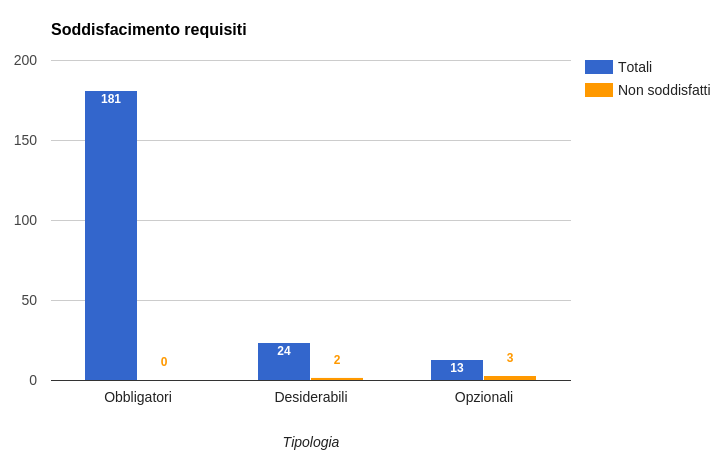
\includegraphics[width=1.1\columnwidth]{immagini/requisiti}
\caption{Soddisfacimento dei requisiti a fine stage}
\label{fig:requisiti-soddisfacimento}%
\end{figure}

\section{Resoconto sugli obiettivi formativi}

I risultati relativi agli obiettivi formativi sono stati riportati nella
tabella \ref{tab:obiettivi-formativi-realizzati}. \\

{
\centering
\begin{tabular}{| p{6cm} | p{6cm} |}

\hline
\textbf{Obiettivo previsto} & \textbf{Risultato} \\
\hline
Ottenimento di una conoscenza profonda di Scrum &
Realizzato \\
\hline
Acquisizione delle competenze necessarie per sviluppare le funzionalità
  previste negli obiettivi produttivi &
Realizzato \\
\hline
Capacità di adattare i principi di Scrum ad esigenze diverse dallo sviluppo
  software &
Parzialmente realizzato \\
\hline
\end{tabular}
\captionof{table}{Obiettivi formativi}
\label{tab:obiettivi-formativi-realizzati}
}
\rule{0pt}{2ex}

L'obiettivo riguardante l'adattamento dei principi di Scrum ad esigenze diverse
dallo sviluppo software è ritenuto parzialmente realizzato per i seguenti
motivi:

\begin{itemize}
\item in parte del tempo speso durante l'ultima settimana e durante lo studio
  della parte di modellazione processi, ho esteso la mia conoscenza riguardo
  la realtà aziendale e ho visto esempi di come Sanmarco Informatica offre il
  proprio \emph{know how} ad aziende di settori diversi dal suo (e.g. a imprese
  che adottano la \emph{lean production} e non Scrum a supporto dei propri
  processi);
\item per ciascuno degli strumenti di \emph{Inspection} è stata valutata la
  possibilità di utilizzare questi nell'ambito dell'analisi di processi nel
  documento in cui essi erano descritti;
\item durante lo studio della metodologia Scrum, diverse fonti contenevano
  informazioni su come i metodi agili fossero nati, di come questi si fossero
  ispirati al \textbf{TPS} (Toyota Production System) e la storia di questo;
\item le funzionalità introdotte sono state sviluppate tenendo conto
  che queste potrebbero essere riusate per scopi diversi dall'applicazione di
  Scrum\footnote{Ad esempio, gli strumenti di \emph{Inspection} possono essere
  visti come mezzi con cui analizzare cicli produttivi di breve durata.}. Hanno
  fatto eccezione il collegamento dell'area Scrum al forum e alla parte di
  modellazione di processi, siccome erano fortemente legate a elementi
  caratteristici di Scrum;
\item durante lo stage gli unici \emph{stakeholder} per l'area Scrum erano i
  componenti del team in cui ero inserito. Di conseguenza, non ho potuto
  verificare se effettivamente quanto ho sviluppato sia concretamente
  utilizzabile per processi di produzione di beni o servizi diversi dal
  software.
\end{itemize}

Riguardo agli obiettivi formativi riportati in tabella
\ref{tab:obiettivi-formativi-realizzati}, ho maturato riflessioni su diversi
aspetti dello stage.

\subsection{Disponibilità del team}

L'apprendimento è stato notevolmente facilitato dalla disponibilità continua
del tutor aziendale e degli altri elementi del team. Infatti ho ricevuto:

\begin{itemize}
\item precise linee guida di sviluppo;
\item aiuto quando ho trovato difficoltà nel procedere con il lavoro;
\item utili consigli su come migliorare l'efficienza per l'esecuzione di
  operazioni SQL e sostegno durante le discussioni per capire quali dati
  estrarre per la creazione di burn-down chart e quale fosse il miglior modo
  per estrarli.
\end{itemize}

\subsection{Comportamento e struttura dell'applicazione Web}

Sebbene non avessi mai utilizzato HTML5 e AngularJS, partivo da una buona
conoscenza di XHTML 1.0 e Javascript ``puro''. Ciò ha influito nel seguente
modo nella mia formazione durante il periodo di stage:

\begin{itemize}
\item HTML5 è un linguaggio che deriva da XHTML. Grazie a questo fattore, mi
  è stato sufficiente individuare le differenze più importanti tra i due per
  non aver grosse difficoltà a sviluppare la parte strutturale delle pagine
  del \FREND;
\item AngularJS è sensibilmente diverso da Javascript. Tuttavia, grazie
  a quanto imparato nel modulo B del corso di Ingegneria del Software, alla
  letteratura utilizzata e alla documentazione trovata su Internet, in breve
  tempo ho potuto far mie alcune delle notevoli possibilità offerte da questo
  \gloss{framework}.
\end{itemize}

\subsection{Architettura del \FREND{}}

Prima dell'attività di stage, non avevo mai sviluppato un'applicazione Web che
fosse contenuta interamente in una sola pagina. Tuttavia, prima dello stage ho
investito parte del mio tempo vedendo come le \gloss{spa} potessero essere
realizzate con AngularJS e le conseguenze che ciò comportava.

In questo modo, ottenere una visione d'insieme dei vari moduli contenuti in
JPA è stato più facile una volta iniziato lo stage.

\subsection{Componente presentazionale di pagine Web}

L'uso di TODC Bootstrap ha semplificato di molto lo sviluppo della parte di
presentazione delle pagine siccome, tramite l'uso di tag o di attributi di
carattere semantico durante la realizzazione della struttura, tale
\gloss{framework} riusciva a fornire lo stile adatto ai vari elementi della
pagina.

\subsection{Gestione delle chiamate \gloss{rest}}

Le \gloss{jaxrs} erano a me nuove e finora non avevo mai utilizzato Java per
la gestione di chiamate \gloss{rest}.

Tuttavia, la semplicità delle \gloss{jaxrs} mi ha permesso di capire in poche
ore come poterle utilizzare e come generare le classi della \emph{business
logic} per ricevere dati con chiamate \gloss{rest} provenienti dal \FREND.

\subsection{Utilizzo di SQL}

Per l'interazione con i \gloss{rdbms} era previsto l'uso di comandi SQL
(linguaggio a me noto già da prima dell'attività di stage) tramite il package
\texttt{java.sql}. Anche se non avevo mai realizzato programmi che includessero
questo package, il suo utilizzo si è rivelato semplice ed intuitivo.

\subsection{Telegram API}

L'obiettivo di mandare notifiche via Telegram è stato aggiunto a stage in
corso.

Quando si è presentata l'ipotesi di implementare un sistema di notifiche con
l'invio di messaggi a dispositivi mobili usando un software già esistente
(Telegram, WhatsApp, Viber, etc.) non avevo alcuna esperienza con tali
sistemi.

Prima di iniziare l'attività, avevo usato Telegram solamente come utente e,
avendo letto le sue FAQ, ero a conoscenza che tale programma rende disponibili
le proprie \gloss{api} per essere utilizzato.

Seguendo solamente la documentazione fornita da Telegram è stato semplice
riuscire a sviluppare in poco tempo le abilità necessarie per implementare le
varie operazioni che il Telegram Bot attualmente offre.

\subsection{Scrum}

Prima dello stage, Scrum e metodi agili per me erano solamente interessanti
campi di studio, poichè non avevo mai avuto modo di poterli vivere sulla mia
pelle come metodologie di lavoro.

Grazie all'attività di stage, ho potuto:

\begin{itemize}
\item capire meglio quali esigenze e quali motivazioni hanno portato le aziende
  ad adottare Scrum;
\item sperimentare una realtà in cui Scrum veniva usato quotidianamente;
\item capire quali benefici derivano dall'applicazione di questo metodo;
\item scoprire delle interessanti attività di supporto a Scrum come il
  \textbf{Planning
  Poker}\footnote{\url{https://en.wikipedia.org/wiki/Planning_poker}};
\item studiare anche i possibili effetti negativi che potrebbero derivare da
  una sua scorretta applicazione e le cause principali di questi.
\end{itemize}

\section{Distanza tra corso di studi e realtà aziendale}

Ad inizio stage non sapevo precisamente quanto di quello che ho visto in Ateneo
avrei trovato in una realtà aziendale come Sanmarco Informatica.

\subsection{Verifica dinamica}

In alcuni insegnamenti universitari viene posta particolare enfasi nel
progettare test per i propri programmi.
Questa attività serve infatti per ridurre la verifica manuale sia da parte di
sviluppatori che di verificatori.

Oltre a notevoli vantaggi in termini di tempo e denaro durante lo sviluppo, i
test automatici portano grandi risparmi quando si tratta di svolgere
manutenzione: cambiando una parte di un programma, è sempre necessario
verificare che tutto il resto funzioni ancora e, nel caso in cui questo
controllo venga eseguito manualmente, ciò costituisce un'intera ripetizione del
ciclo di verifica dinamica.

Tuttavia, nella realtà industriale che ho conosciuto questa pratica non è
diffusa anche se il suo impiego avrebbe probabilmente comportato guadagni per
l'azienda.

\subsection{UML}

Nell'insegnamento di Ingegneria del Software vengono visti diversi tipi di
diagramma \gloss{uml} per vari scopi: definizione degli scenari possibili di un
programma, analisi della sua esecuzione, analisi della sua architettura o
dell'interazione fra componenti, etc.

Per quanto ho potuto vedere, a livello industriale non tutti gli strumenti
tecnologici visti nel mondo accademico sono presenti o utilizzati: ad esempio
spesso è preferita la realizzazione di mockup o spiegazioni di tipo discorsivo
sul lavoro che bisogna svolgere.

Durante lo stage, l'introduzione di strumenti come i diagrammi \gloss{uml} ha
permesso di esprimere più chiaramente alcuni concetti discussi con gli
\emph{stakeholder}, rimuovendo ambiguità e fornendo di fatto uno strumento
efficace per il dialogo.

\subsection{Design pattern}

All'interno di JPA non ho notato l'uso di \gloss{design-pattern}, a meno che
questi non siano direttamente imposti o implementati nativamente dai
\gloss{framework} utilizzati.

Per quanto ho potuto vedere, ad esempio nel progetto di Ingegneria del
Software, i \gloss{design-pattern} costituiscono invece una componente
fondamentale per architetture di sistemi informatici, poichè garantiscono
diverse qualità ed evitano di incorrere nei cosiddetti \emph{anti-pattern},
come ad esempio il già menzionato \gloss{telescoping}.

\subsection{Strumenti e procedure per la qualità}

In tutti gli insegnamenti universitari in cui fosse previsto un progetto o la
realizzazione di un programma per il superamento dell'esame, ho notato che
veniva posta particolare attenzione ad alcune qualità specifiche per ogni
materia di studio.

Durante l'attività di stage non ho invece notato particolari strumenti che
imponessero il rispetto di standard di tipo qualitativo, se non le norme e le
raccomandazioni adottate dal team di sviluppo.

Di conseguenza, ho semplicemente cercato di perseguire le qualità viste
all'Università affinchè architettura e codice fossero facilmente estendibili e
comprensibili con i seguenti accorgimenti:

\begin{itemize}
\item uso di pre-condizioni, post-condizioni e invarianti nei frammenti di
  codice più complessi;
\item uso di Javadoc;
\item uso di \gloss{design-pattern} architetturali;
\item contenimento della complessità ciclomatica e del numero dei livelli di
  annidamento;
\item limitazione della lunghezza dei metodi e del numero di parametri per
  metodo;
\item incapsulazione, poichè la maggior parte delle classi preesistenti aveva
  i campi dati degli oggetti ad accesso pubblico, mentre per le classi di
  package di mia creazione ho ristretto l'accesso a tali membri delle entità.
\end{itemize}

\subsection{Tecnologie emergenti}

A differenza di molte startup o aziende consolidate, durante la mia esperienza
all'Università ho avuto raramente a che fare con tecnologie emergenti o
innovative.

Molti insegnamenti infatti si basano su tecnologie considerate stabili e,
dal momento che sono usate frequentemente dalle aziende, ciò comporta che sia
per progetti didattici che per lo svolgimento di esami vengano impiegate
solamente quelle.

Se da un lato può costituire senza dubbio una garanzia in termini di
prospettiva occupazionale, dall'altro è vero che quando ho affrontato lo stage
mi trovavo ad utilizzare per la prima volta tecnologie recenti ed attualmente
diffuse come AngularJS o Bootstrap\footnote{Al momento della stesura della
tesi, il \gloss{framework} originale (non quello proposto da TODC) è il
progetto con più preferenze, ovvero 86583 utenti, su GitHub.}.

Un altro esempio possono essere Python e Ruby on Rails: questi linguaggi,
comunemente diffusi a livello industriale, non vengono mai discussi in alcun
corso (se non incidentalmente in alcuni progetti di Ingegneria del Software).

\subsection{Importanza degli insegnamenti}

Il fatto di aver completato anticipatamente gli obiettivi mi ha fatto capire
ancor di più quanto l'Università prepari i propri studenti non tanto a
specializzarsi per essere uno sviluppatore di un certo linguaggio, ma ad
essere una figura professionale in grado di adattarsi e avente conoscenze tali
da poter affrontare problemi con molta facilità.

Ritengo infatti che i seguenti insegnamenti abbiano contribuito
significativamente alla buona riuscita dello stage:

\begin{itemize}
\item \textbf{Ingegneria del Software:} questo insegnamento e il relativo
  progetto mi hanno permesso di acquisire delle conoscenze e competenze che si
  sono rivelate molto utili, tra cui:
  \begin{itemize}
  \item conoscenza di Scrum e confronto di questa metodologia con altri modelli
    di sviluppo software;
  \item uso di sistemi di versionamento e l'analisi sulle varie modalità di
    impiego di questi;
  \item conoscenza di qualità da ricercare per architetture e codice sorgente;
  \item capacità di produrre documenti di natura uniforme tra loro e riuso
    sistematico di documenti sviluppati precedentemente;
  \item conoscenza ed uso dei diagrammi \gloss{uml};
  \item individuazione di norme e raccomandazioni a supporto dei processi di
    sviluppo;
  \item \gloss{best-practice} per le attività di analisi e progettazione;
  \item uso dei \gloss{design-pattern}.
  \end{itemize}
\item \textbf{Programmazione e Algoritmi e Strutture Dati:} le abilità
  acquisite in questi insegnamenti mi hanno permesso di affrontare facilmente
  le complessità algoritmiche dovute a:
  \begin{itemize}
  \item preparazione dei dati per i burn-down chart: era necessario un
    algoritmo che fosse efficiente e capace di soddisfare tutti i requisiti
    fissati;
  \item realizzazione del linguaggio per le notifiche: questo problema è stato
    affrontato con raffinamenti successivi di uno dei semplici algoritmi di
    ricerca di occorrenze in un testo visti nel corso di Programmazione.
  \end{itemize}
\item \textbf{Programmazione ad oggetti:} questo insegnamento mi ha permesso
  di capire a fondo i principi cardine della programmazione ad oggetti;
\item \textbf{Programmazione concorrente e distribuita:} con questo
  insegnamento ho appreso le \gloss{best-practice} e le caratteristiche più
  importanti di Java, linguaggio largamente usato durante l'attività di stage;
\item \textbf{Data Mining:} le conoscenze acquisite in questo insegnamento,
  inserito a libera scelta nel piano di studi, mi hanno aiutato principalmente
  in due occasioni:
  \begin{itemize}
  \item realizzazione della curva di carico ``reale'' nei burn-down chart;
  \item analisi critica dei dati presenti nei vari strumenti di
    \emph{Inspection} e capacità di descrivere cosa si può ricavare da questi.
  \end{itemize}
\item \textbf{Tecnologie Web:} insegnamento in cui viene posta molta attenzione
  sull'accessibilità dei siti Web e sulla buona realizzazione di struttura e
  presentazione di questi. Ha favorito l'apprendimento delle varie tecnologie
  per il \FREND;
\item \textbf{Basi di dati:} dal momento che durante lo stage ho dovuto
  progettare tabelle e realizzare delle interrogazioni per ricavare dati da
  queste, l'insegnamento mi ha fornito le giuste basi teoriche e pratiche per
  poter effettuare entrambe le attività.
\end{itemize}

\subsection{Collaborazione studenti-professori}

A differenza di altre università, nel Corso di Laurea triennale vi sono poche
iniziative che coinvolgono attivamente studenti e professori.

Questo aspetto è a mio parere limitante per le possibilità che l'Università
degli Studi di Padova potrebbe offrire, visto che attività del genere
potrebbero fornire sia dell'utile \emph{know-how} come preparazione per il
mondo del lavoro, che interessanti spunti su svariati campi di ricerca.

\subsection{Progetti didattici}

Alcuni progetti durante il corso di studi sono di tipo \emph{one-off}, infatti
forniscono una serie di conoscenze che rischiano di rimanere isolate e non
integrate con il resto degli insegnamenti. Altri, più complessi, riescono a
fornire conoscenze che sono riutilizzabili in un secondo momento.

Secondo me, la possibilità di svolgere progetti più impegnativi è
un'opportunità per lo studente di sviluppare una base solida di abilità
considerevoli da poter spendere nel mondo del lavoro.

Un'attività che nel corso degli anni portasse a realizzare un'applicazione che
consideri tutte le tematiche trattate nei vari insegnamenti porterebbe con sè
un bagaglio di competenze altamente significativo.
             % Valutazione retrospettiva
\appendix
%\input{capitoli/capitolo-A}             % Appendice A

%**************************************************************
% Materiale finale
%**************************************************************
\backmatter
\printglossary[title={Glossario}]
% !TEX encoding = UTF-8
% !TEX TS-program = pdflatex
% !TEX root = ../tesi.tex
% !TEX spellcheck = it-IT

%**************************************************************
% Bibliografia
%**************************************************************

\cleardoublepage
\chapter{Indice delle fonti}

\nocite{*}
%\printbibliography

\bibbycategory % equivale a dare un \printbibliography per ogni categoria


\end{document}
